\documentclass[11pt]{article}

% ----------------------------------------------------------------------
%  Mixed Traffic Flow and Edge AI-Supported V2I Communication in
%  Intelligent Transportation Systems via CARLA Simulation
%  Taha Yasin Er, Doruk Topcu  --  Hacettepe University, CMP 764
%  Single-column article. Compile on Overleaf with pdfLaTeX + BibTeX.
% ----------------------------------------------------------------------

\usepackage[utf8]{inputenc}
\usepackage[T1]{fontenc}
\usepackage[a4paper,margin=1in]{geometry}
\usepackage{graphicx}
\usepackage{booktabs}
\usepackage{amsmath,amssymb}
\usepackage{caption}
\usepackage{subcaption}
\usepackage{xcolor}
\usepackage{enumitem}
\usepackage{array}
\usepackage{float}
\usepackage[hidelinks]{hyperref}

\graphicspath{{figures/}}
\captionsetup{font=small,labelfont=bf}
\setlength{\parskip}{0.35em}

\title{\vspace{-1.0em}\textbf{Mixed Traffic Flow and Edge AI-Supported V2I Communication
in Intelligent Transportation Systems via CARLA Simulation}\\[0.45em]
\large A CARLA Study of Combined V2I/V2V Cooperative Perception with ETSI CPM
Release~2 under Realistic 5G~NR-V2X Channel and Edge-Compute Constraints}

\author{Taha Yasin Er \qquad Doruk Topcu\\[0.3em]
Department of Computer Engineering, Hacettepe University\\
\texttt{CMP\,764 -- Final Project}}

\date{June 2026}

\begin{document}
\maketitle

\begin{abstract}
\noindent Line-of-sight occlusions at urban intersections are a primary obstacle for
automated driving: even the best on-board sensors cannot see through buses,
buildings, or foliage. Cooperative Perception (CP) addresses this through an
Internet-of-Things architecture in which infrastructure and vehicles share what
they observe over a vehicular network. We present \textbf{V2X-Sim}, an end-to-end
cooperative-perception framework built in CARLA~0.9.16 that, unlike idealized CP
datasets, transmits standardized \mbox{ETSI~TS\,103\,324} Collective Perception
Messages (CPM, Release~2, ASN.1~UPER) across a \emph{realistic} 5G~NR-V2X channel
governed by the Coll-Perales latency model and the Thandavarayan packet-delivery
model with an endogenous channel-busy-ratio feedback loop. Roadside Units (RSUs)
run a fine-tuned YOLO26s detector under an edge-compute budget; each Connected
Autonomous Vehicle (CAV) fuses incoming messages with a time-aware late-fusion
tracker, a confirmation-hysteresis filter, and a time-to-collision (TTC) braking
ladder. Crucially, the framework now supports \textbf{three communication arms}---%
Combined (V2I$+$V2V), V2I-only, and V2V-only---enabling a clean ablation of where
the safety benefit originates. We run a 144-cell sweep (3 arms $\times$ 4
penetration rates $\times$ 3 maps $\times$ 2 weather presets $\times$ 2 seeds) in
dense, hostile, NHTSA-anchored mixed traffic (60 vehicles $+$ 60 pedestrians). The
headline result is a clean, monotonic safety gain: mean collisions fall from
$\sim$22 (all-human baseline) to $\sim$6 at full cooperative penetration---a
$\sim$73\% reduction---on every arm and every map, with a consistent ordering
\mbox{Combined $\leq$ V2I-only $\leq$ V2V-only}, identifying infrastructure CPM as
the stronger single channel. Map complexity sets the collision floor and the
safety curve is robust to heavy rain. We additionally report sensitivity findings
from an earlier experimental configuration (detector cross-map bottleneck,
traffic-density saturation, and a low-sun ``ClearSunset paradox''). An interactive
demonstration application is described in Appendix~\ref{app:demo}.
\end{abstract}

% ======================================================================
\section{Introduction}
% ======================================================================
The transition toward autonomous urban mobility is fundamentally bottlenecked by
the physical limits of on-board sensing. Even advanced vehicle-mounted LiDAR and
optical suites cannot penetrate buildings, large vehicles, or dense foliage at
intersections, leaving safety-critical blind spots exactly where vulnerable road
users (VRUs) are most exposed. To mitigate these line-of-sight occlusions,
Intelligent Transportation Systems (ITS) research has pivoted toward
\emph{Cooperative Perception} (CP)---an Internet-of-Things (IoT) architecture in
which infrastructure sensors and connected vehicles share their observations so
that a vehicle can ``see'' a hazard it has no direct line of sight to.

The purpose of this work is to evaluate the safety benefit of cooperative
perception under \emph{realistic}, constrained conditions. Rather than assuming
instantaneous, lossless communication, we integrate true edge-compute limits and
5G~NR-V2X channel degradation (latency and packet loss) and ask how the system
performs in hostile, chaotic traffic, adverse weather, and pedestrian-dense
environments. Our previous study modeled only the infrastructure-to-vehicle (V2I)
channel; the present version additionally models vehicle-to-vehicle (V2V)
exchange and supports running V2I, V2V, or both together, so that the origin of
the safety benefit can be isolated by ablation.

We compose the ecosystem from state-of-the-art tools:
\begin{itemize}[leftmargin=1.3em,itemsep=0.15em,topsep=0.2em]
  \item \textbf{CARLA Simulator (0.9.16)}~\cite{carla2017} --- a high-fidelity 3D
  environment with ground-truth physics and a configurable, hostile human-driver
  Traffic Manager.
  \item \textbf{Ultralytics YOLO26s}~\cite{ultralytics2024} --- a specialized,
  multi-weather object detector fine-tuned for intersection camera geometry.
  \item \textbf{ASN.1 / asn1tools} --- to compile and strictly enforce the ETSI
  ASN.1 standard for Collective Perception Messages.
  \item \textbf{A parametric 5G~NR-V2X channel} --- a deterministic in-process
  broker that imposes the Coll-Perales latency and Thandavarayan packet-delivery
  models, with a 1\,s channel-busy-ratio (CBR) feedback loop.
\end{itemize}

\noindent\textbf{Contributions.}
(i) A literature-grounded experimental harness that, for the first time, composes
an empirical YOLO26s perception pipeline, ETSI CPM Release~2 payloads, the
Coll-Perales/Thandavarayan channel models, edge-compute bounds, and
NHTSA-anchored human drivers inside one CARLA-physics loop.
(ii) A time-aware late-fusion CAV module with message-age compensation and a
three-rule confirmation hysteresis that suppresses phantom braking.
(iii) A three-arm (V2I/V2V/Combined) penetration ablation across maps, weather,
and seeds that yields a clean, monotonic safety law and isolates the
infrastructure channel as the dominant contributor.
(iv) An interactive demonstration application (Appendix~\ref{app:demo}).

% ======================================================================
\section{Related Work}
% ======================================================================
Cooperative-perception research has largely evolved along two disparate paths:
idealized perception simulators and abstracted communication models.

\noindent\textbf{Prior simulators.} Frameworks such as OPV2V~\cite{opv2v2022} and
V2X-Sim (NYU)~\cite{v2xsim2022} have made major contributions by providing
standardized datasets for training collaborative perception models (e.g.\ fusing
multi-agent point clouds). However, these studies overwhelmingly evaluate under
the assumption of an ideal, zero-latency channel in which packets are never lost.
Hao et al.'s \emph{RCooper} benchmark~\cite{rcooper2024} adds strong external
validity that \emph{late fusion} (transmitting bounding boxes rather than raw
point clouds) outperforms early fusion at real intersections because of sensor
heterogeneity, motivating our message-level design. OpenCDA~\cite{opencda2021} and
V2X-ViT~\cite{v2xvit2022} similarly target the fusion model rather than the
channel.

\noindent\textbf{Channel modeling.} Conversely, telecommunications studies have
rigorously modeled the 5G~NR-V2X channel. The Coll-Perales latency
model~\cite{collperales2022} provides a foundational decomposition of end-to-end
V2X delay into transmission, propagation, queuing, and processing terms. Likewise,
Thandavarayan et al.~\cite{thandavarayan2020} provide CPM generation rules and a
packet-delivery-ratio (PDR) model for collective perception, and NR sidelink
surveys~\cite{ahangar2023} situate these in the broader standard. These works,
however, abstract the perception layer away entirely, treating vehicles as Poisson
message generators rather than agents reacting to visual stimuli.

\noindent\textbf{Our relation to the literature.} This work bridges the seam left
between the two camps. By composing an empirically derived YOLO26s pipeline with
the Coll-Perales/Thandavarayan channel models and edge-compute bounds, we
\emph{invert} the traditional setup: the realistic channel becomes the
experimental treatment, while the cooperative-perception accuracy and the
resulting collision outcomes inside the CARLA physics engine are the measured
responses.

% ======================================================================
\section{Methodology and System Architecture}
% ======================================================================
\subsection{System overview}
Figure~\ref{fig:arch} shows the end-to-end pipeline. Two perception sources feed
every CAV. On the \emph{infrastructure} (V2I) path, an RSU camera frame is run
through YOLO26s, back-projected to world coordinates, encoded into an ETSI CPM,
and published to the channel. On the \emph{vehicle} (V2V) path, a peer CAV
broadcasts a compact cooperative message carrying its own perceived objects and a
hard-brake intent flag. Both message types traverse the same parametric
5G~NR-V2X channel (latency, packet loss, channel load) and are fused late inside
the receiving CAV, which evaluates time-to-collision and, if warranted, issues a
braking override. An interactive application that visualizes this pipeline live is
described in Appendix~\ref{app:demo}.

\begin{figure}[t]
  \centering
  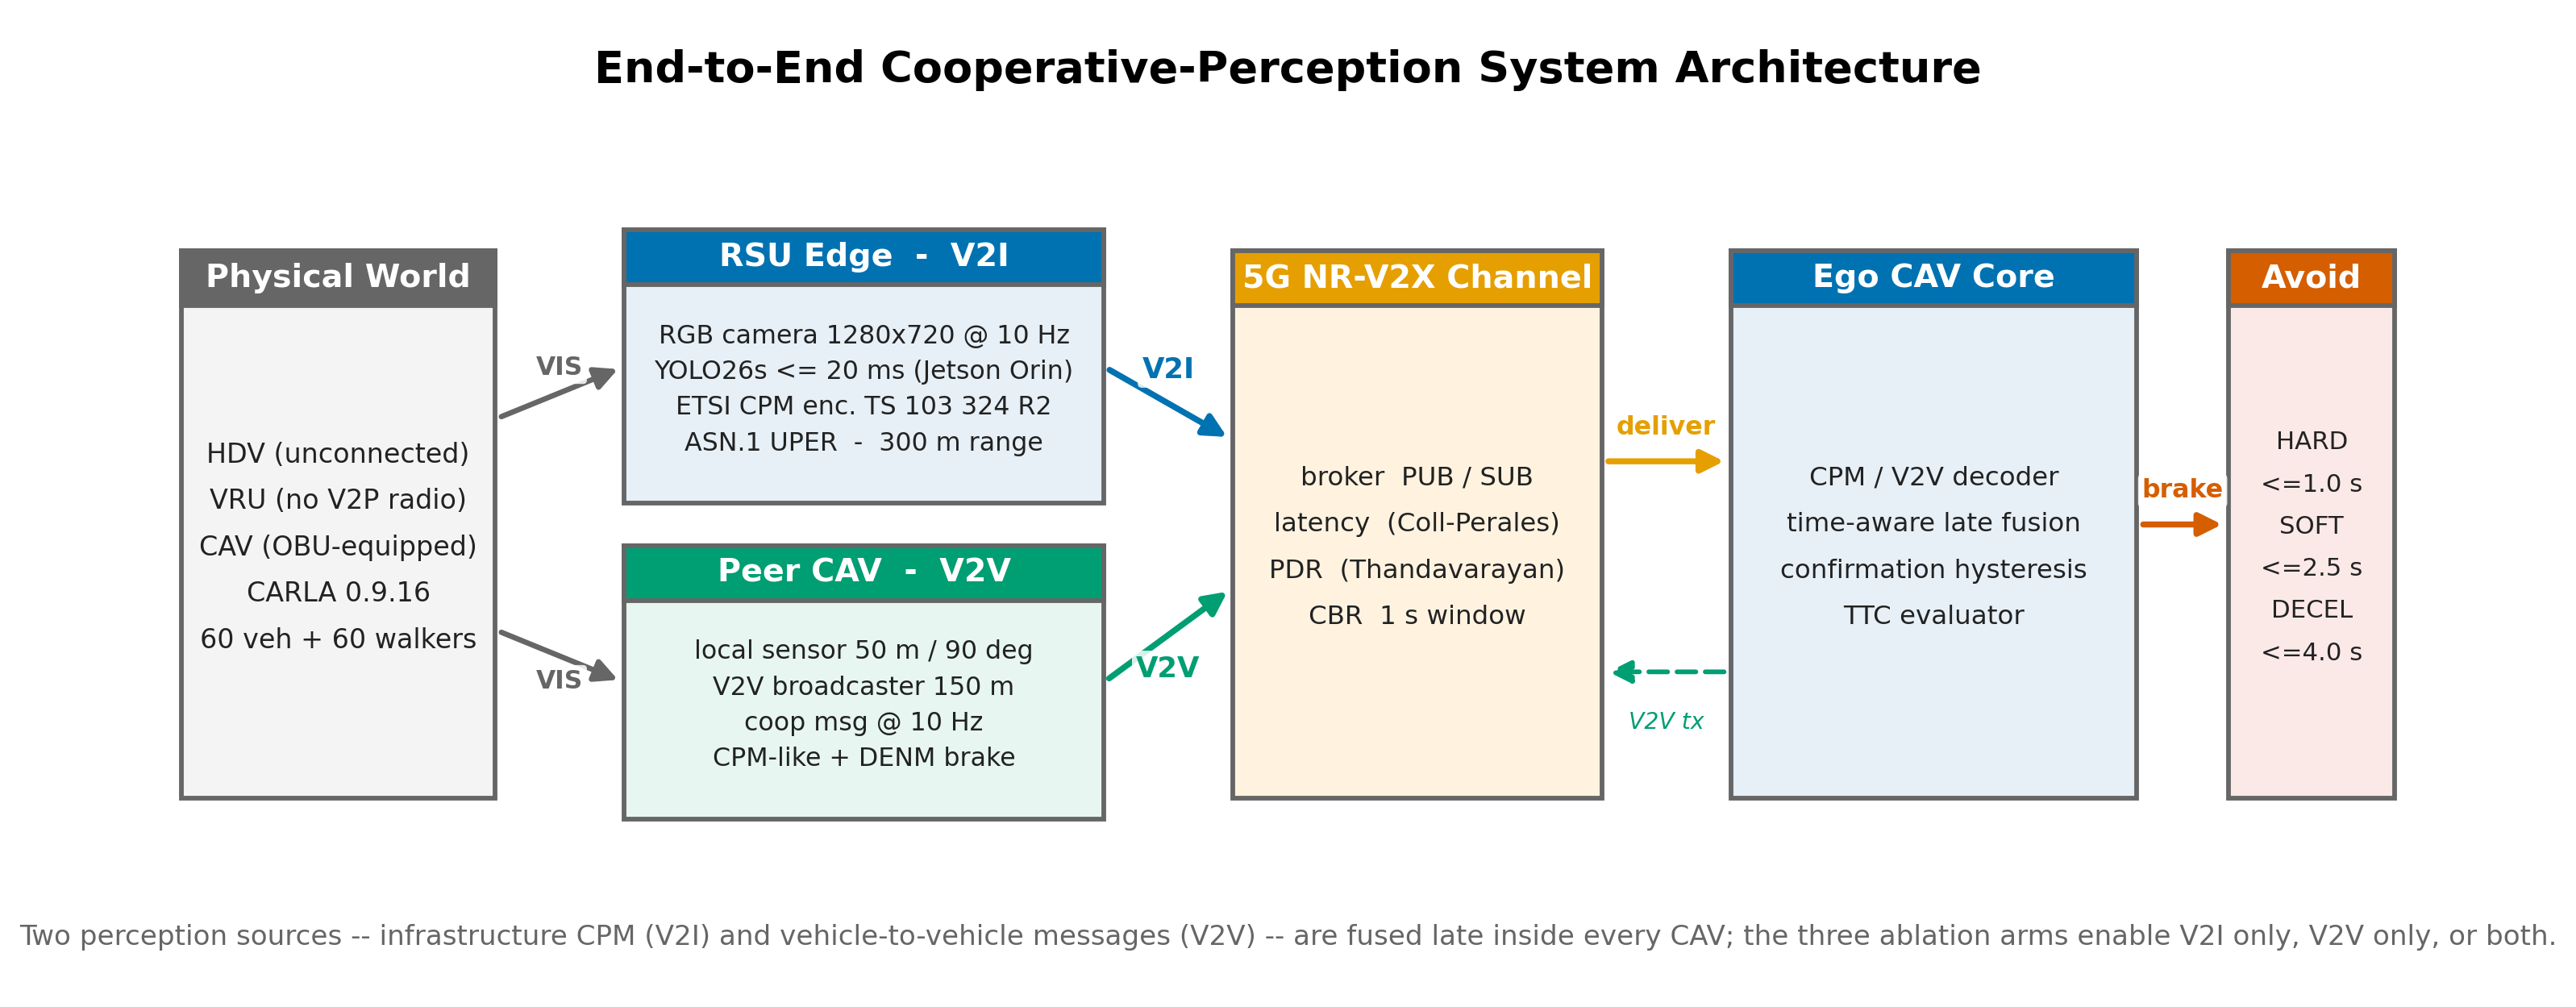
\includegraphics[width=\textwidth]{fig01-architecture.png}
  \caption{End-to-end cooperative-perception architecture. Infrastructure CPM
  (V2I) and vehicle-to-vehicle messages (V2V) are fused late inside every CAV; the
  three ablation arms enable V2I only, V2V only, or both.}
  \label{fig:arch}
\end{figure}

\subsection{Roadside perception and edge compute}
Each RSU carries a single RGB camera ($1280\times720$, $90^\circ$ FOV) mounted on a
traffic-light pole and pitched down toward the junction. Frames are processed at
10\,Hz by a YOLO26s detector. Detections are filtered by confidence
($\geq 0.25$) and class, and the bottom-centre of each bounding box is
back-projected onto the ground plane ($z=0$) to recover a world position. The
detector is fine-tuned for a four-class taxonomy
(\texttt{vehicle}, \texttt{motorcycle}, \texttt{bicycle}, \texttt{pedestrian}).
The RSU perception loop enforces a strict edge-compute budget---e.g.\ $20$\,ms per
frame on a Jetson AGX~Orin, $50$\,ms on a Xavier---above which frames are dropped,
propagating missing or stale objects into the stream as a graceful-degradation
mechanism.

\subsection{CPM encoding (ETSI Release 2)}
Hazards are serialized strictly to the ETSI \mbox{TS\,103\,324} Release~2
standard~\cite{etsicpm2023} using ASN.1 \mbox{UPER} (header
\texttt{protocolVersion}=2,
\texttt{messageId}=14), with the Common Data Dictionary~\cite{etsicdd}. Each
perceived object carries class, relative position and velocity (in centimetre/%
centimetre-per-second units), and a quantized confidence
($\mathrm{INTEGER}(0..101)$). YOLO classes map onto ETSI categories
(\texttt{passengerCar}, \texttt{motorcyclist}, \texttt{pedalCycle},
\texttt{pedestrian}); the payload is capped at $1100$ bytes, and the encoded byte
length drives the channel transmission time.

\subsection{5G NR-V2X channel models}
Both V2I and V2V messages traverse the same deterministic, in-process broker that
imposes three coupled models.

\noindent\emph{Latency (Coll-Perales~\cite{collperales2022}).} The end-to-end
delay of a message of size $s$ bytes over distance $d$ at channel load $\rho$ is
\begin{equation}
T_{\mathrm{e2e}} = T_{\mathrm{proc}}^{\mathrm{tx}} + T_{\mathrm{tx}}(s)
   + T_{\mathrm{prop}}(d) + T_{\mathrm{queue}}(\rho) + T_{\mathrm{proc}}^{\mathrm{rx}},
\end{equation}
with $T_{\mathrm{tx}}=\lceil 8s/B_{\mathrm{slot}}\rceil\,\tau_{\mathrm{slot}}$,
$T_{\mathrm{prop}}=d/c$, and $T_{\mathrm{queue}}=\kappa\rho$, plus additive
Gaussian jitter $\mathcal{N}(0,\sigma^2)$. We use the ``realistic'' profile
(processing times after 3GPP~TS\,38.214~\cite{tgpp38214};
$T_{\mathrm{proc}}^{\mathrm{tx}}=T_{\mathrm{proc}}^{\mathrm{rx}}=2$\,ms,
$\tau_{\mathrm{slot}}=0.5$\,ms, $B_{\mathrm{slot}}=4000$\,bits,
$\kappa=10$\,ms, $\sigma=5$\,ms), giving 5G~NR-V2X-like single-digit-millisecond
delays.

\noindent\emph{Packet delivery (Thandavarayan~\cite{thandavarayan2020}).} Each
broadcast is delivered to each receiver as a Bernoulli trial with success
probability
\begin{equation}
P_{\mathrm{succ}}(d,\rho) = \bigl(1-\alpha\rho\bigr)\,
   \exp\!\Bigl[-\bigl(d/d_{\mathrm{ref}}\bigr)^{\gamma}\Bigr],
\end{equation}
with $d_{\mathrm{ref}}=220$\,m, $\gamma=2$, $\alpha=0.3$
($\approx$81\% delivery at 100\,m on an idle channel). Release~2 broadcasts are
unacknowledged, so there is no retransmission.

\noindent\emph{Channel load (CBR).} The channel-busy ratio
$\rho(t)=\bigl(\sum T_{\mathrm{tx}}\ \text{in window}\bigr)/W$ is measured over a
$W=1000$\,ms sliding window and fed back into both the latency and PDR models,
making channel load endogenous to message volume.

\subsection{V2I, V2V, and the three communication arms}
Figure~\ref{fig:topo} shows the network topology. Infrastructure CPMs flow from
RSUs to in-range CAVs (PC5 range $300$\,m); cooperative V2V messages flow between
CAVs ($150$\,m range) and additionally carry a declared hard-brake intent
(a DENM-like hazard signal). HDVs carry no radio and are perceived only. The
framework toggles which links are active to realize three arms:
\textbf{V2I-only} (RSU CPM only), \textbf{V2V-only} (CAV$\leftrightarrow$CAV only),
and \textbf{Combined} (both). All three share the identical channel model, so the
arm comparison is a clean treatment.

\begin{figure}[t]
  \centering
  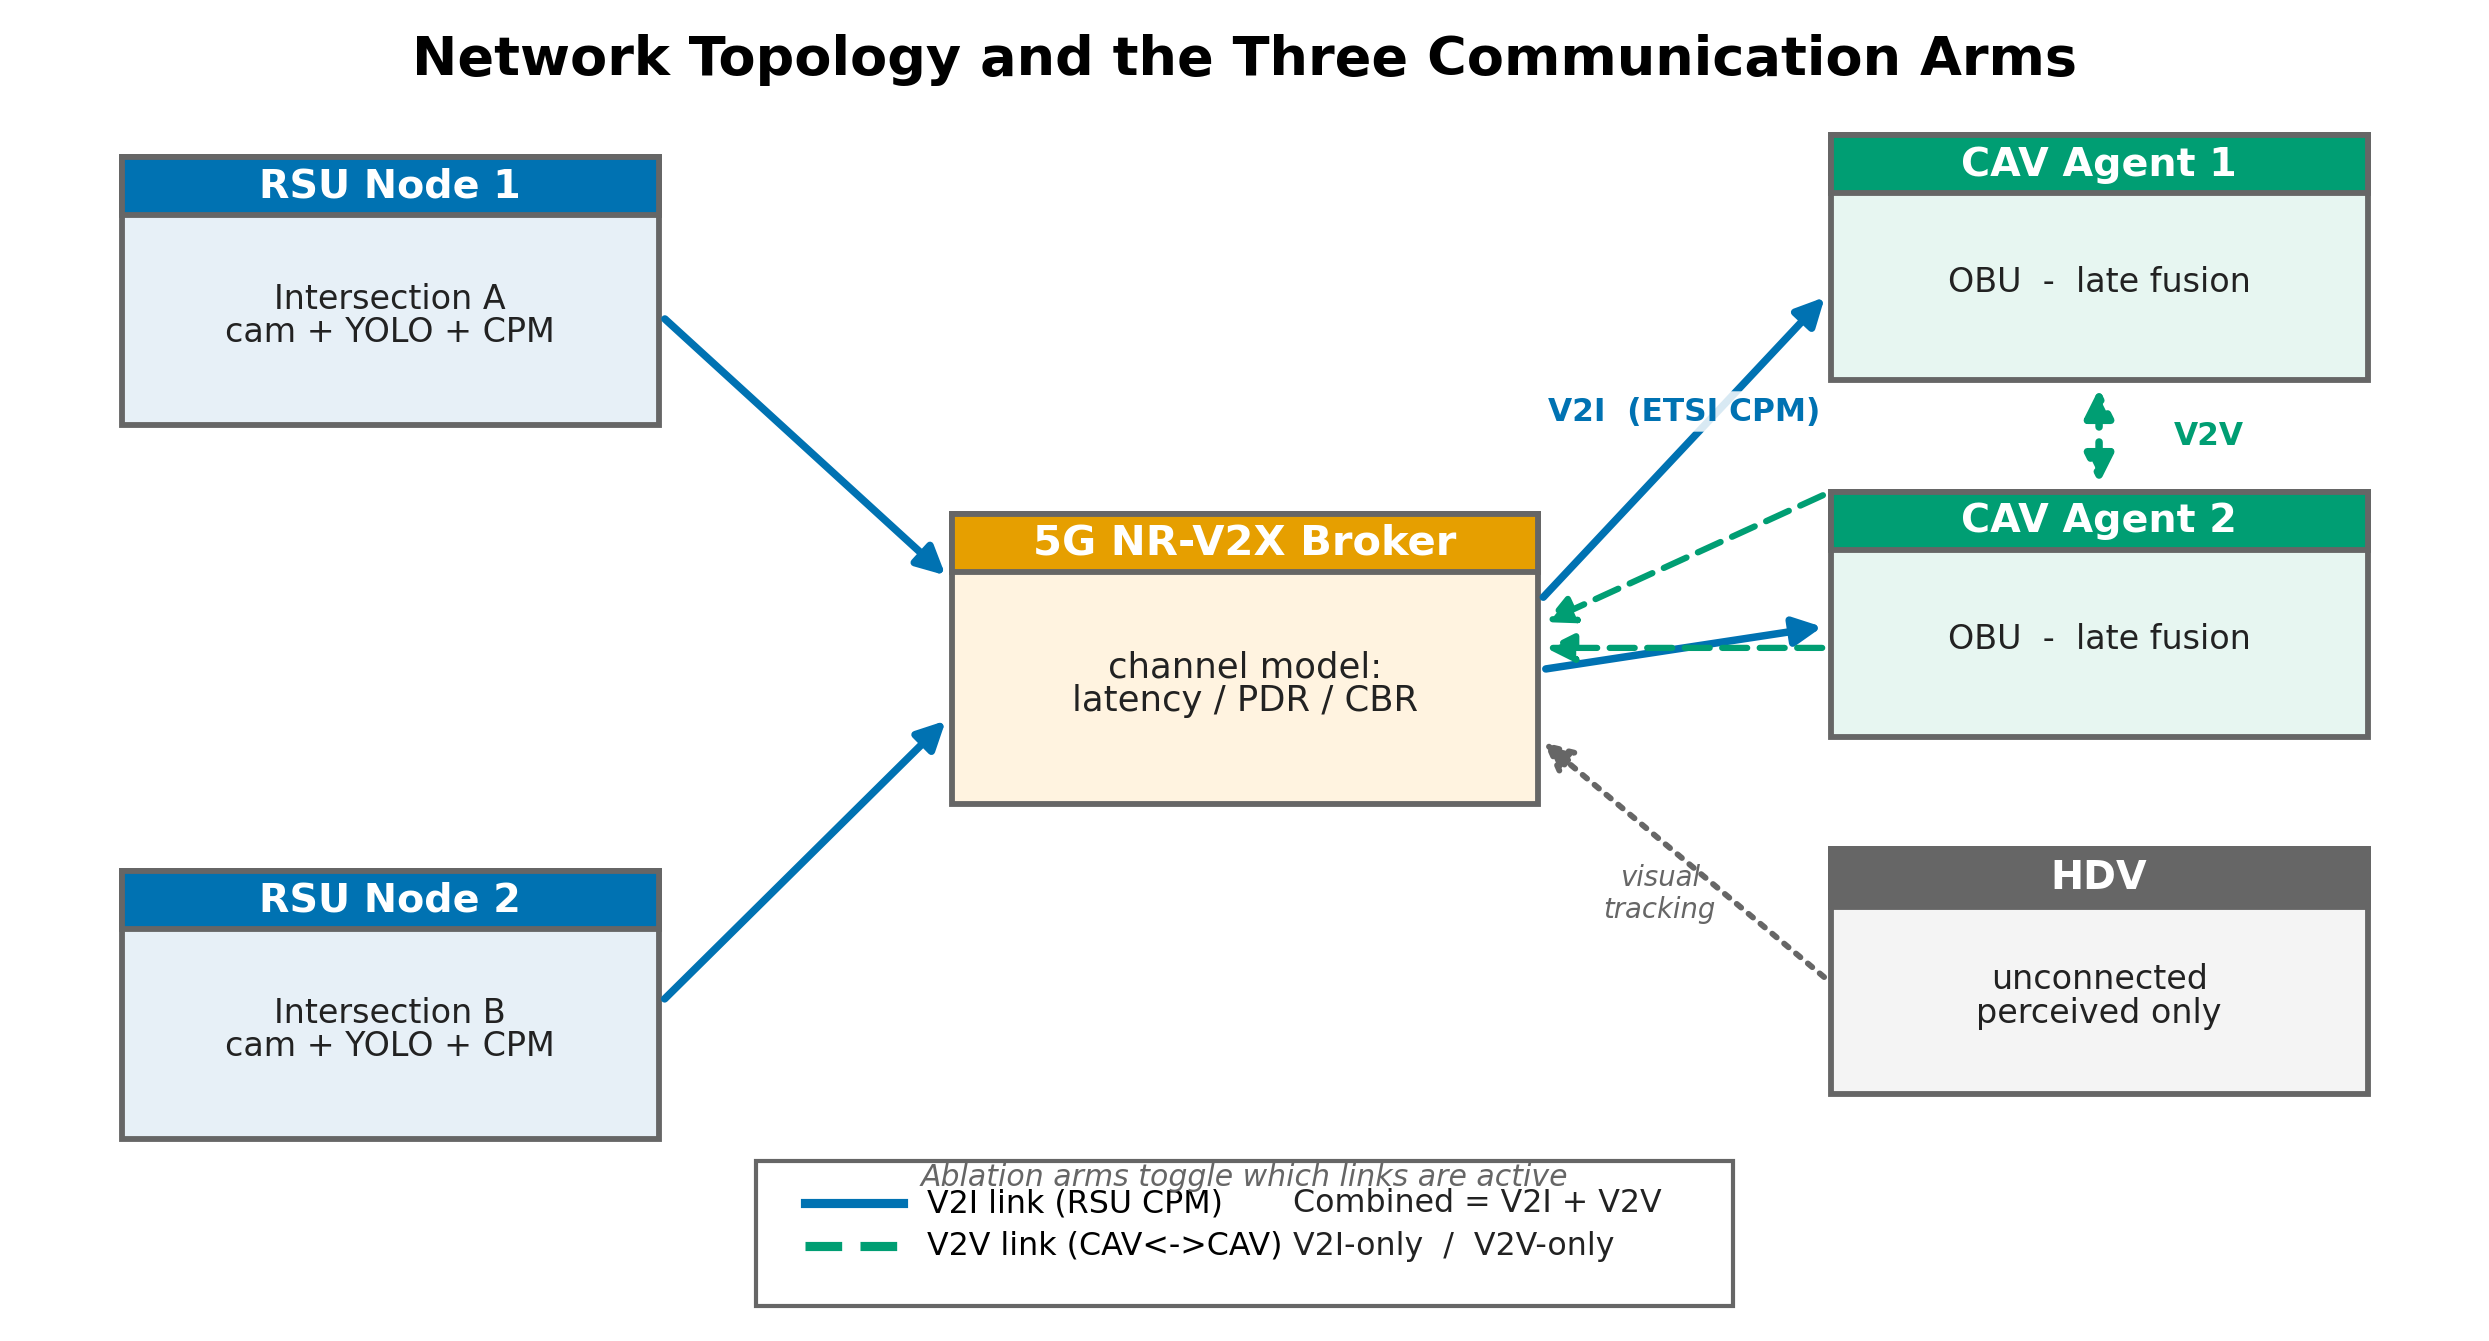
\includegraphics[width=\textwidth]{fig02-topology.png}
  \caption{Network topology and the three communication arms. V2I links carry RSU
  CPMs; V2V links carry CAV-to-CAV cooperative messages; HDVs are unconnected. The
  ablation arms enable V2I only, V2V only, or both.}
  \label{fig:topo}
\end{figure}

\subsection{CAV time-aware late fusion and hysteresis}
Each CAV maintains a set of object tracks. An incoming CPM/V2V object is
transformed to world coordinates, \emph{forward-propagated} at constant velocity
by its message age ($\Delta t = t_{\mathrm{now}}-t_{\mathrm{sent}}$) to compensate
for channel delay, and its confidence is linearly decayed over a $1000$\,ms track
lifetime. Objects are matched to existing tracks by a $5$\,m gated nearest-neighbour
association (class must match), and the ego excludes its own ghost reflections by a
velocity-matched self-exclusion test.

To prevent a single spurious detection from triggering emergency braking, a track
may actuate the brakes only if it is \emph{confirmed} by at least one of:
(a)~the CAV's own local sensor; (b)~two observations from a single RSU; or
(c)~two distinct RSUs within a $500$\,ms window. Unconfirmed tracks are retained
for awareness but cannot brake; a would-be brake that is blocked this way is logged
as a \emph{suppressed phantom brake}. Confirmed tracks are graded against a TTC
ladder:
\textsc{hard\,brake} if $\mathrm{TTC}\leq 1.0$\,s and confidence $\geq 0.8$;
\textsc{soft\,brake} if $\mathrm{TTC}\leq 2.5$\,s and confidence $\geq 0.6$;
\textsc{decelerate} if $\mathrm{TTC}\leq 4.0$\,s and confidence $\geq 0.4$.
A declared V2V hard-brake from a leader within $40$\,m and the forward cone
bypasses perception hysteresis as a trusted self-report. The brake override is
applied for a single tick and, critically, \emph{preserves the Traffic Manager's
steering} so a braking CAV does not arc wide mid-turn.

\subsection{Human-driver and VRU models}
Without heterogeneous drivers, CARLA's default Traffic Manager (TM) produces
essentially zero collisions. We therefore assign NHTSA-anchored~\cite{nhtsa2024}
driver profiles (Table~\ref{tab:profiles}). The ablation uses the
\textsc{hostile\_mix} (50\% attentive / 20\% distracted / 30\%
aggressive-hostile): \emph{attentive} drivers keep TM collision avoidance and are
essentially never at fault, whereas \emph{distracted} and \emph{aggressive-hostile}
drivers run with avoidance \emph{off}, so their own rule-violation rates generate
an attributable conflict gradient. CAVs use a deliberately non-oracle
\textsc{ai\_realistic} profile (a long $7$\,m headway, $\sim$1\% residual
violation, avoidance on) on top of the cooperative-perception decision layer.
Pedestrians (VRUs) walk at NHTSA-anchored speeds ($1.4\pm0.3$\,m\,s$^{-1}$, clipped
to $[0.5,2.5]$) and cross the roadway with $\sim$50\% probability, producing
realistic vehicle--pedestrian conflict geometry.

\begin{table}[t]
  \centering
  \caption{Driver profiles pushed into the CARLA Traffic Manager. Percentages are
  the fraction of decision events in which the rule is ignored; speed is signed
  relative to the limit. The ablation uses the hostile mix (top three rows); CAVs
  use the \textsc{ai\,realistic} profile.}
  \label{tab:profiles}
  \small
  \begin{tabular}{lcccccccc}
    \toprule
    Profile & Share & Speed & Follow & Ign.\ lights & Ign.\ signs
            & Ign.\ veh. & Ign.\ walk. & TM avoid. \\
            & (\%)  & $\Delta$\% & (m) & (\%) & (\%) & (\%) & (\%) & \\
    \midrule
    Attentive            & 50 & $0$   & 2.5 & 0  & 0  & 0  & 0  & ON  \\
    Distracted           & 20 & $-10$ & 2.0 & 5  & 10 & 20 & 10 & OFF \\
    Aggressive-hostile   & 30 & $+25$ & 2.0 & 50 & 60 & 40 & 20 & OFF \\
    \midrule
    CAV (AI-realistic)   & -- & $0$   & 7.0 & 1  & 1  & 0  & 0  & ON  \\
    \bottomrule
  \end{tabular}
\end{table}

% ======================================================================
\section{Experimental Design}
% ======================================================================
We executed a full \textbf{144-cell} ablation (Table~\ref{tab:grid}): three
communication arms $\times$ four penetration rates $\times$ three maps $\times$
two weather presets $\times$ two seeds. Each cell simulates $90$\,s at a fixed
$0.05$\,s timestep (20\,Hz) with 60 vehicles and 60 pedestrians; CPM/V2V broadcast
cadence is $100$\,ms (10\,Hz). At penetration $p=0$ the fleet is 100\% human, so no
V2X/V2V is used---this column is the shared all-human baseline, identical across
arms up to CARLA run-to-run nondeterminism. The two seeds were executed on two
machines and merged. Each statistic below is a mean over the \textbf{12 cells} that
share an (arm, penetration) pair (2 seeds $\times$ 3 maps $\times$ 2 weather);
error bars and ``$\pm$'' denote one standard deviation across those 12 cells.

\begin{table}[t]
  \centering
  \caption{Ablation grid (144 cells).}
  \label{tab:grid}
  \small
  \begin{tabular}{ll}
    \toprule
    Dimension & Values \\
    \midrule
    Communication arm & Combined (V2I$+$V2V), V2I-only, V2V-only \\
    Penetration $p$ & 0.0, 0.5, 0.9, 1.0 \\
    Map & Town01 (grid), Town05 (multi-lane), Town10HD (downtown) \\
    Weather & ClearNoon, HardRainNoon \\
    Seeds & 0, 1 (two machines) \\
    Traffic & 60 vehicles $+$ 60 pedestrians; hostile driver mix \\
    Duration & 90\,s/cell @ $dt=0.05$\,s; CPM/V2V @ 10\,Hz \\
    \bottomrule
  \end{tabular}
\end{table}

\noindent\textbf{Metrics.} A \emph{collision} is a de-duplicated incident (one per
unordered vehicle pair within a 1\,s window). \emph{Primary} collisions exclude
secondary pile-ups into an already-immobilized wreck. We further attribute each
incident by party (CAV / HDV / VRU), by at-fault driver profile, and tally CAV
evasive actions, suppressed phantom brakes, cooperative (V2V-triggered) brakes,
delivered V2V messages, emitted CPMs, and immobilized (``frozen'') vehicles.

% ======================================================================
\section{Results and Discussion}
% ======================================================================
\subsection{Detector validation}
Before evaluating the end-to-end channel, the YOLO26s detector was validated to
ensure baseline competency (Figure~\ref{fig:detector}, Table~\ref{tab:detector}).
On in-distribution validation (Town03/04/05) it reaches mAP@50~$=0.757$; on the
held-out Town10HD it drops to mAP@50~$=0.534$. The detector is intentionally tuned
to a \emph{high-precision, moderate-recall} operating point
($\approx$0.85 cross-town precision): every spurious detection is channel noise
and a potential phantom brake, so precision is favoured. This 0.22 mAP gap across
map topologies is the central explanatory factor behind the cross-map sensitivity
discussed in Section~\ref{sec:additional}. The cross-town confusion matrix
(Figure~\ref{fig:cm}) shows the residual error concentrates among the visually
similar two-wheeler classes and missed (background) detections, consistent with the
moderate-recall operating point.

\begin{figure}[t]
  \centering
  \begin{subfigure}{0.48\textwidth}
    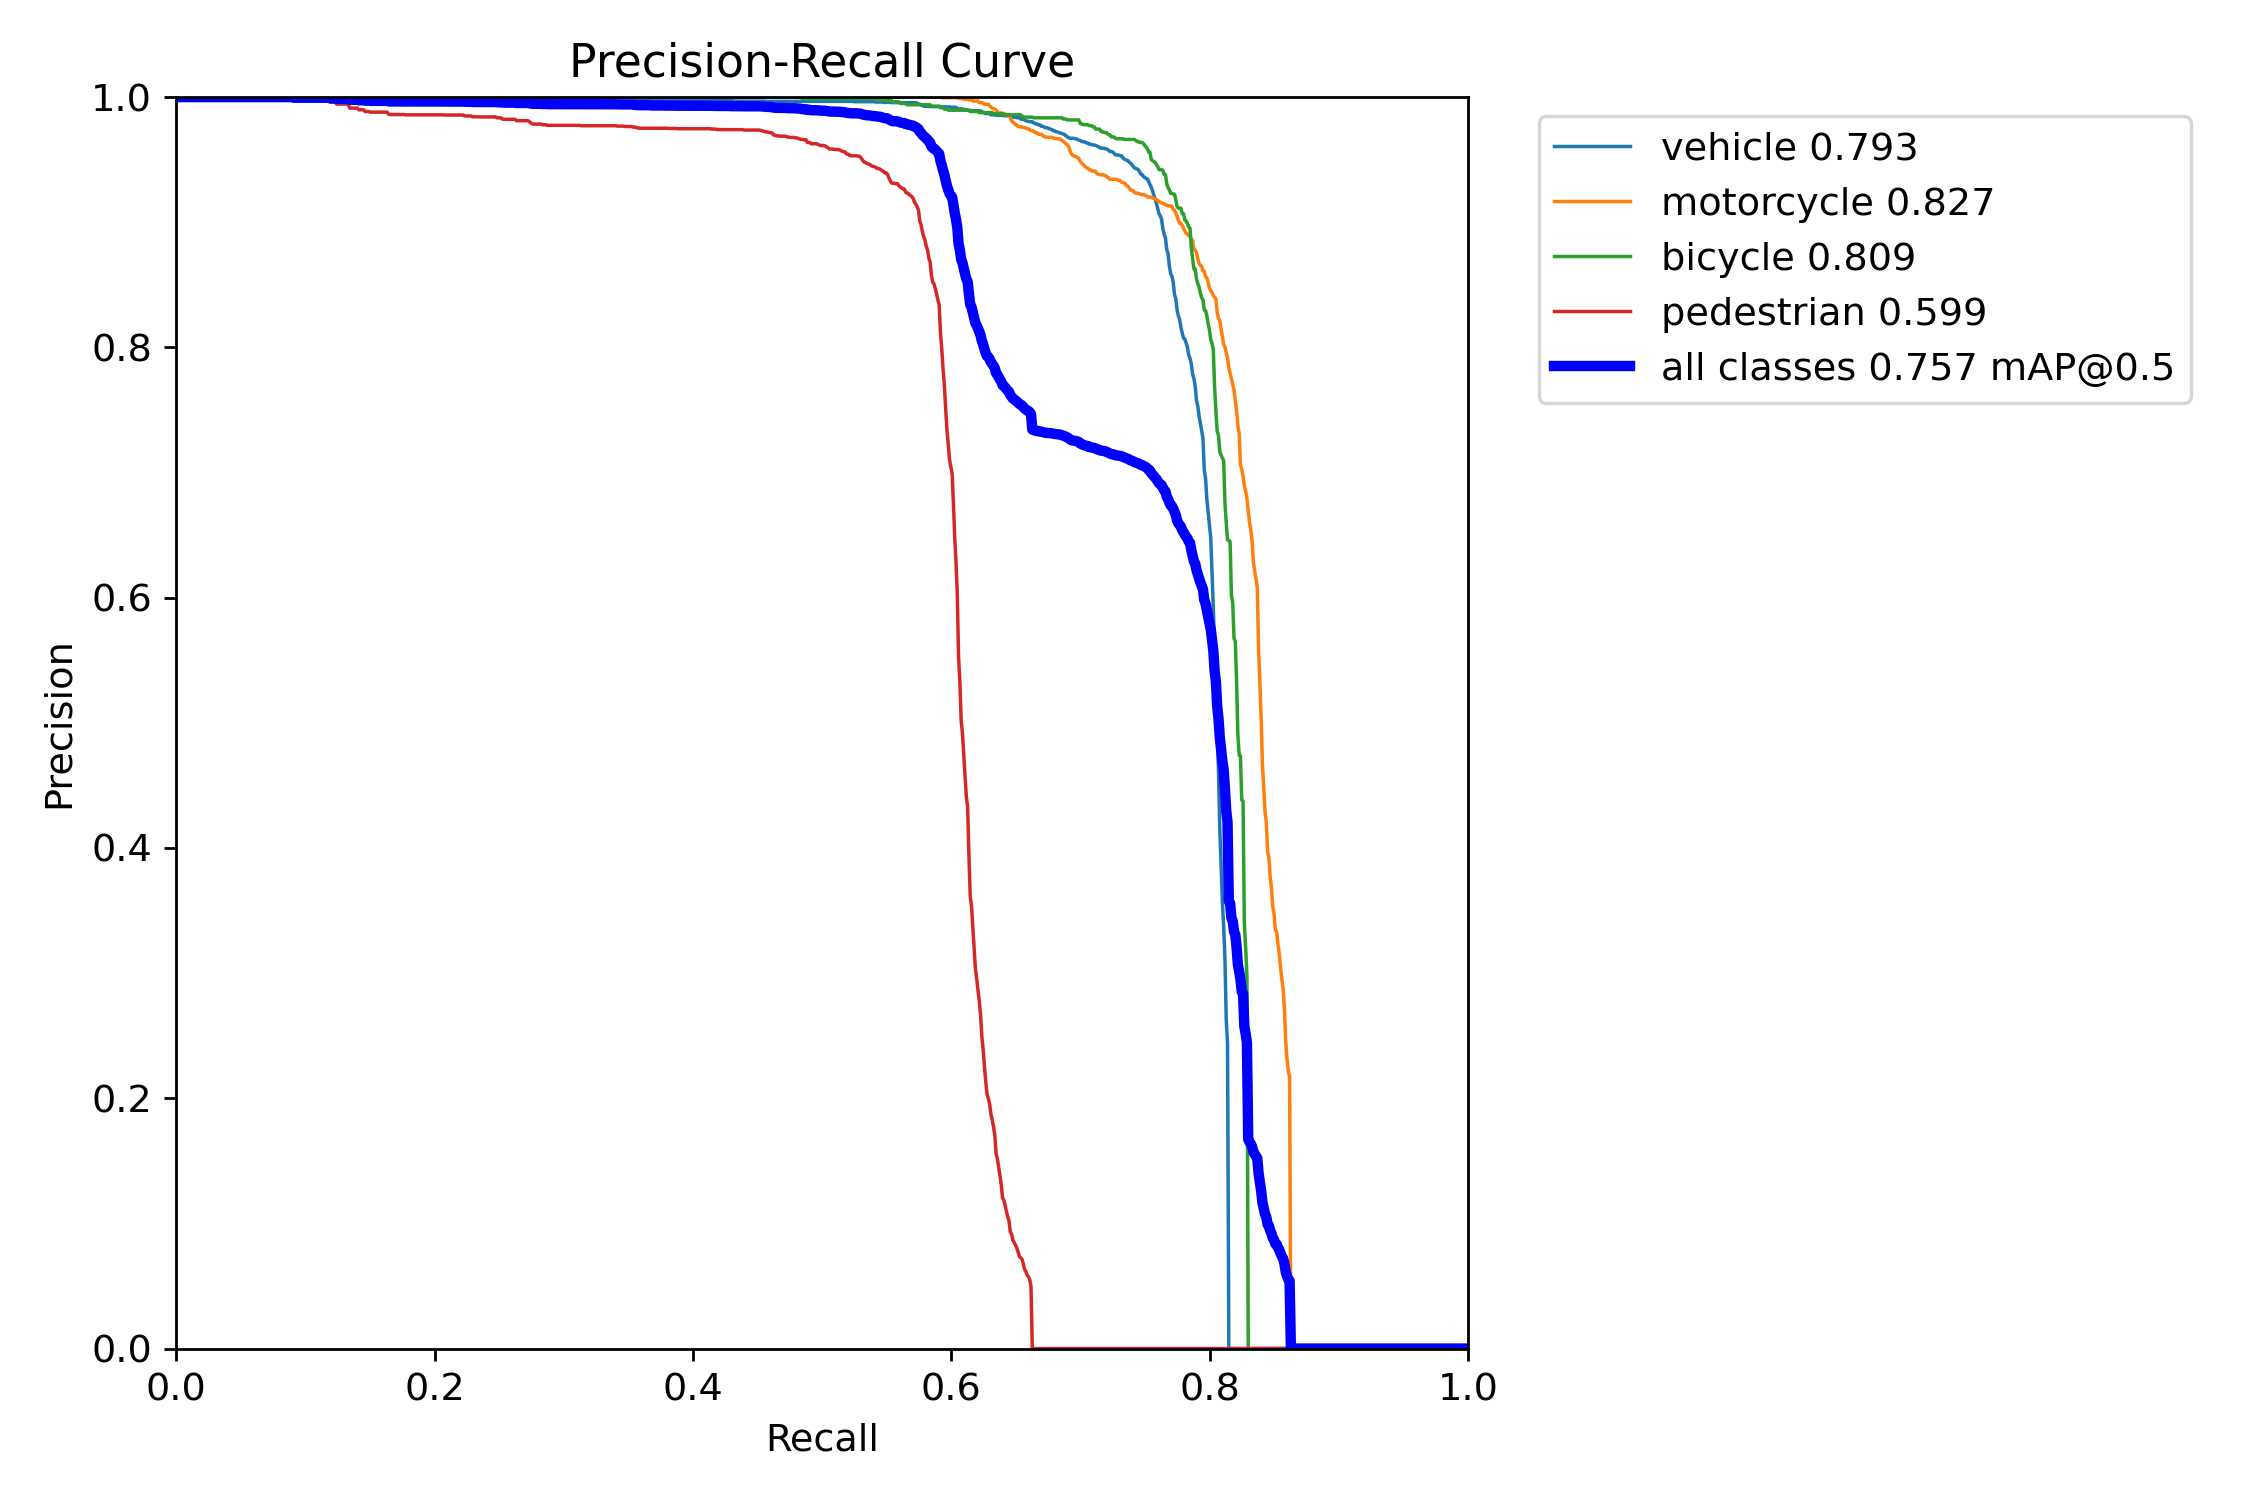
\includegraphics[width=\linewidth]{fig13-detector-pr-indist.png}
    \caption{In-distribution (Town03/04/05).}
  \end{subfigure}\hfill
  \begin{subfigure}{0.48\textwidth}
    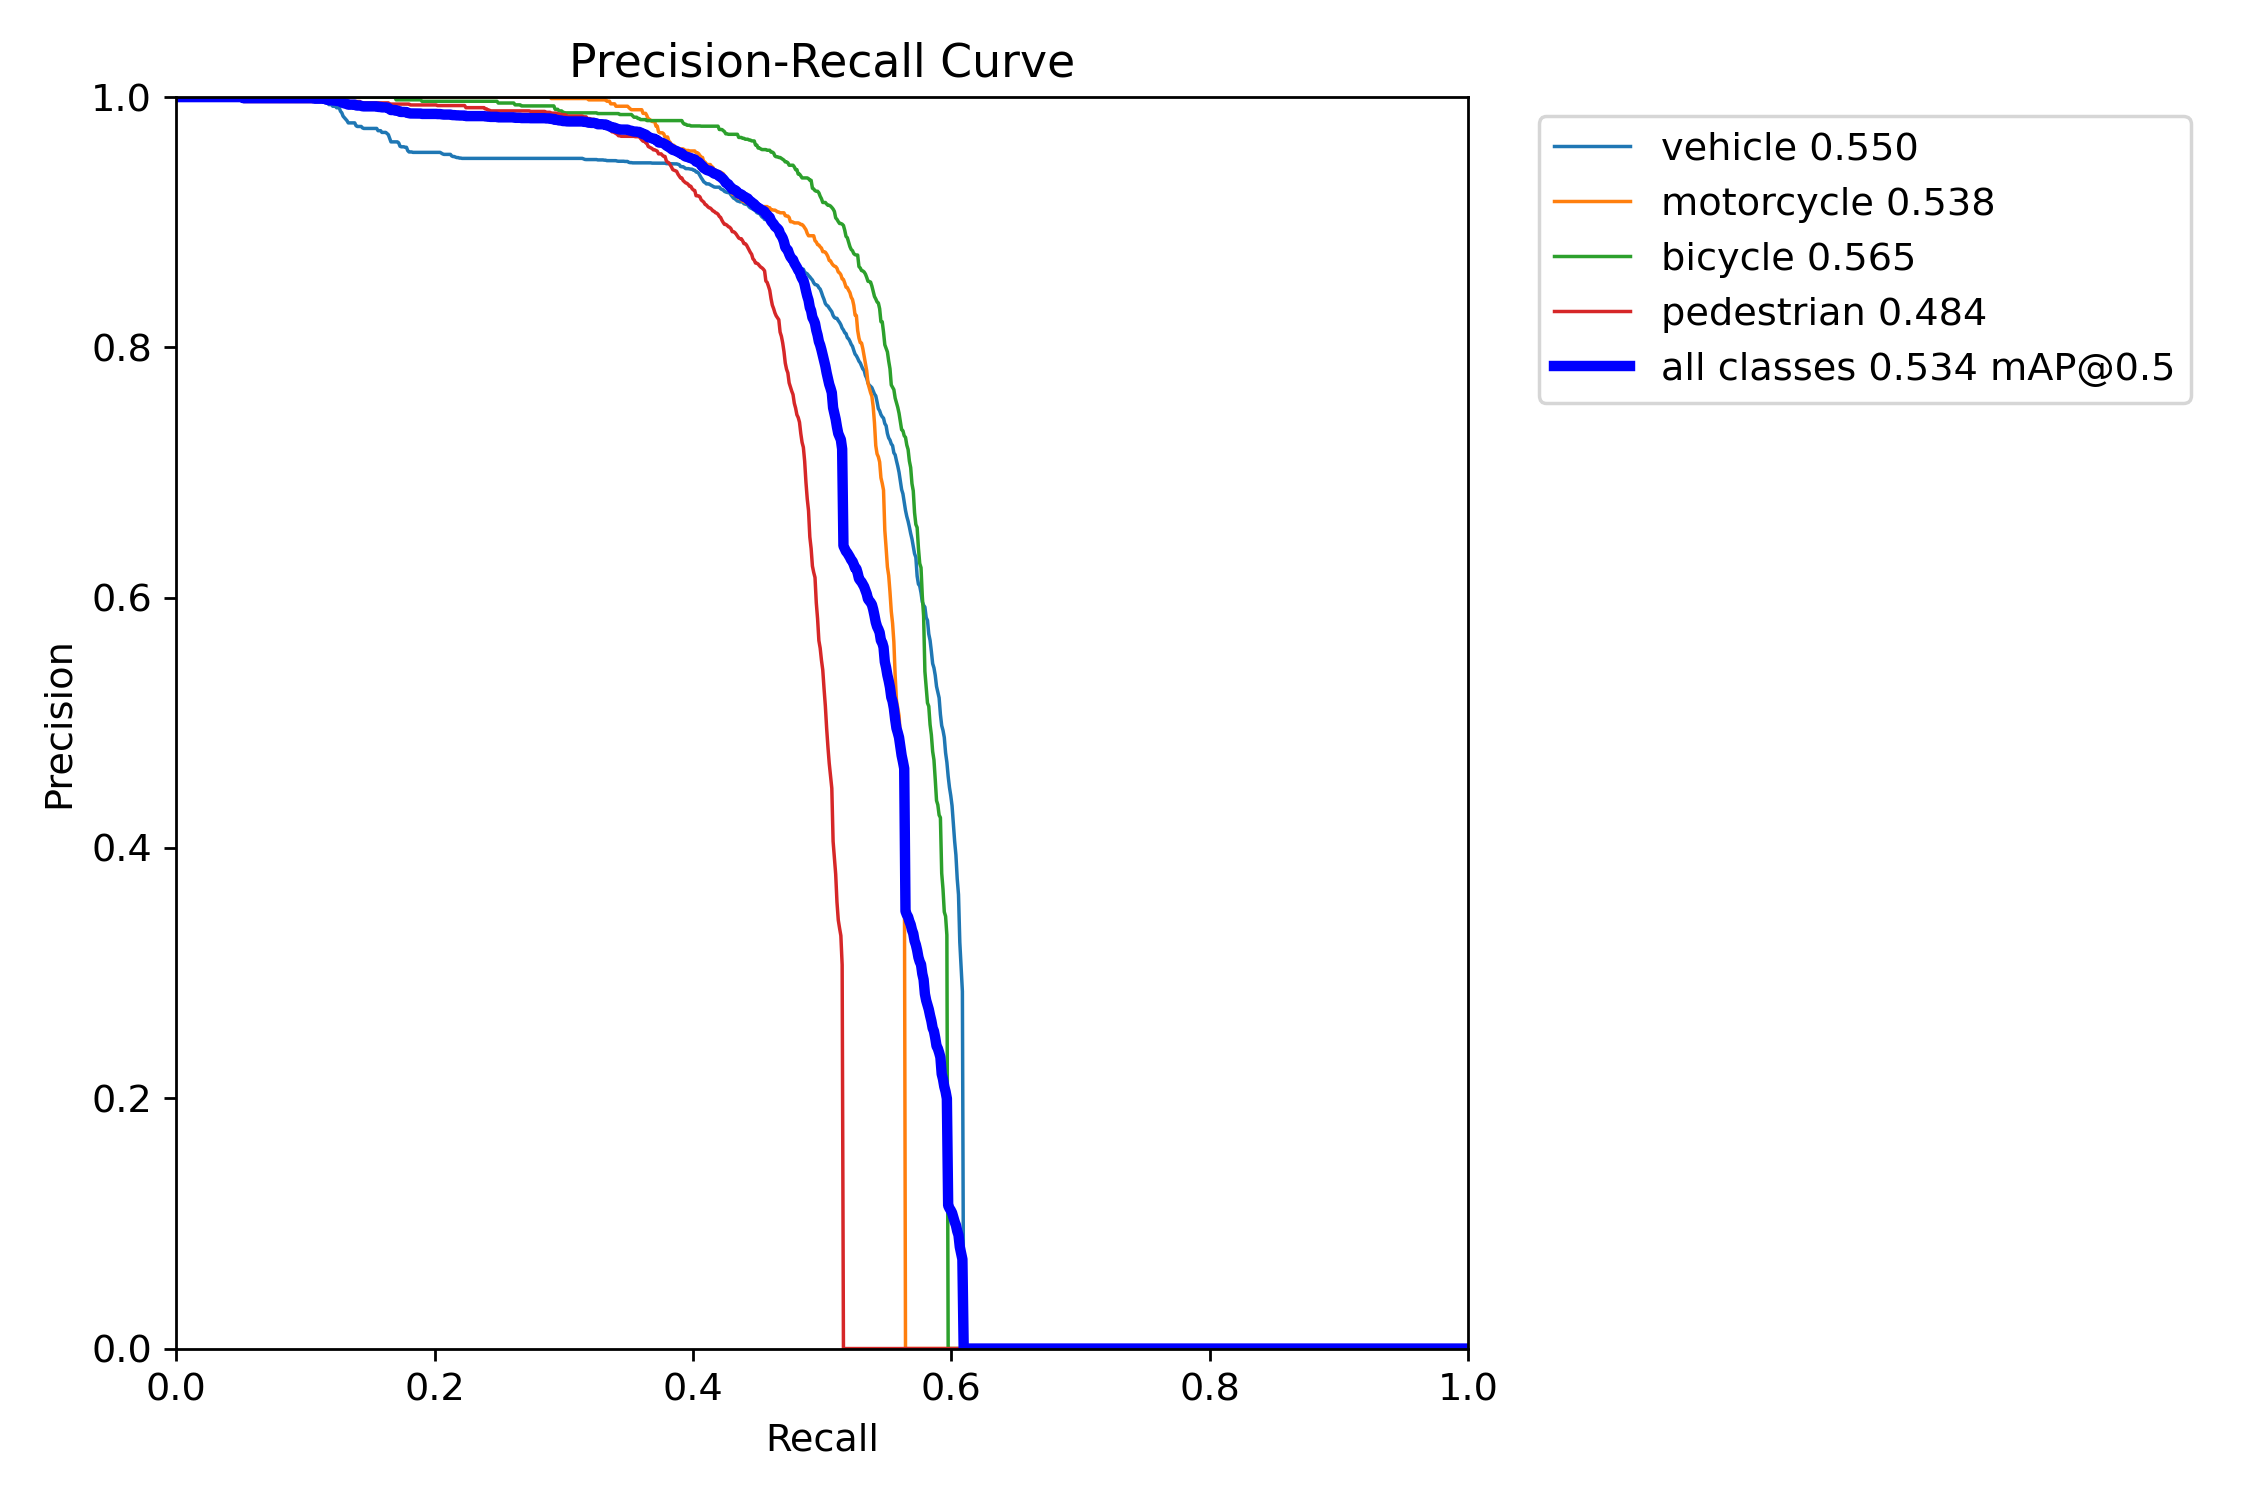
\includegraphics[width=\linewidth]{fig14-detector-pr-town10.png}
    \caption{Cross-town (held-out Town10HD).}
  \end{subfigure}
  \caption{YOLO26s precision--recall curves. The cross-town collapse bounds the
  achievable cooperative-perception benefit on unseen map topologies.}
  \label{fig:detector}
\end{figure}

\begin{table}[t]
  \centering
  \caption{Detector metrics: in-distribution vs.\ cross-town.}
  \label{tab:detector}
  \small
  \begin{tabular}{lcccc}
    \toprule
    Split & Precision & Recall & mAP@50 & mAP@50:95 \\
    \midrule
    In-distribution (Town03/04/05) & 0.926 & 0.712 & 0.757 & 0.610 \\
    Cross-town (Town10HD)          & 0.852 & 0.500 & 0.534 & 0.369 \\
    \bottomrule
  \end{tabular}
\end{table}

\begin{figure}[t]
  \centering
  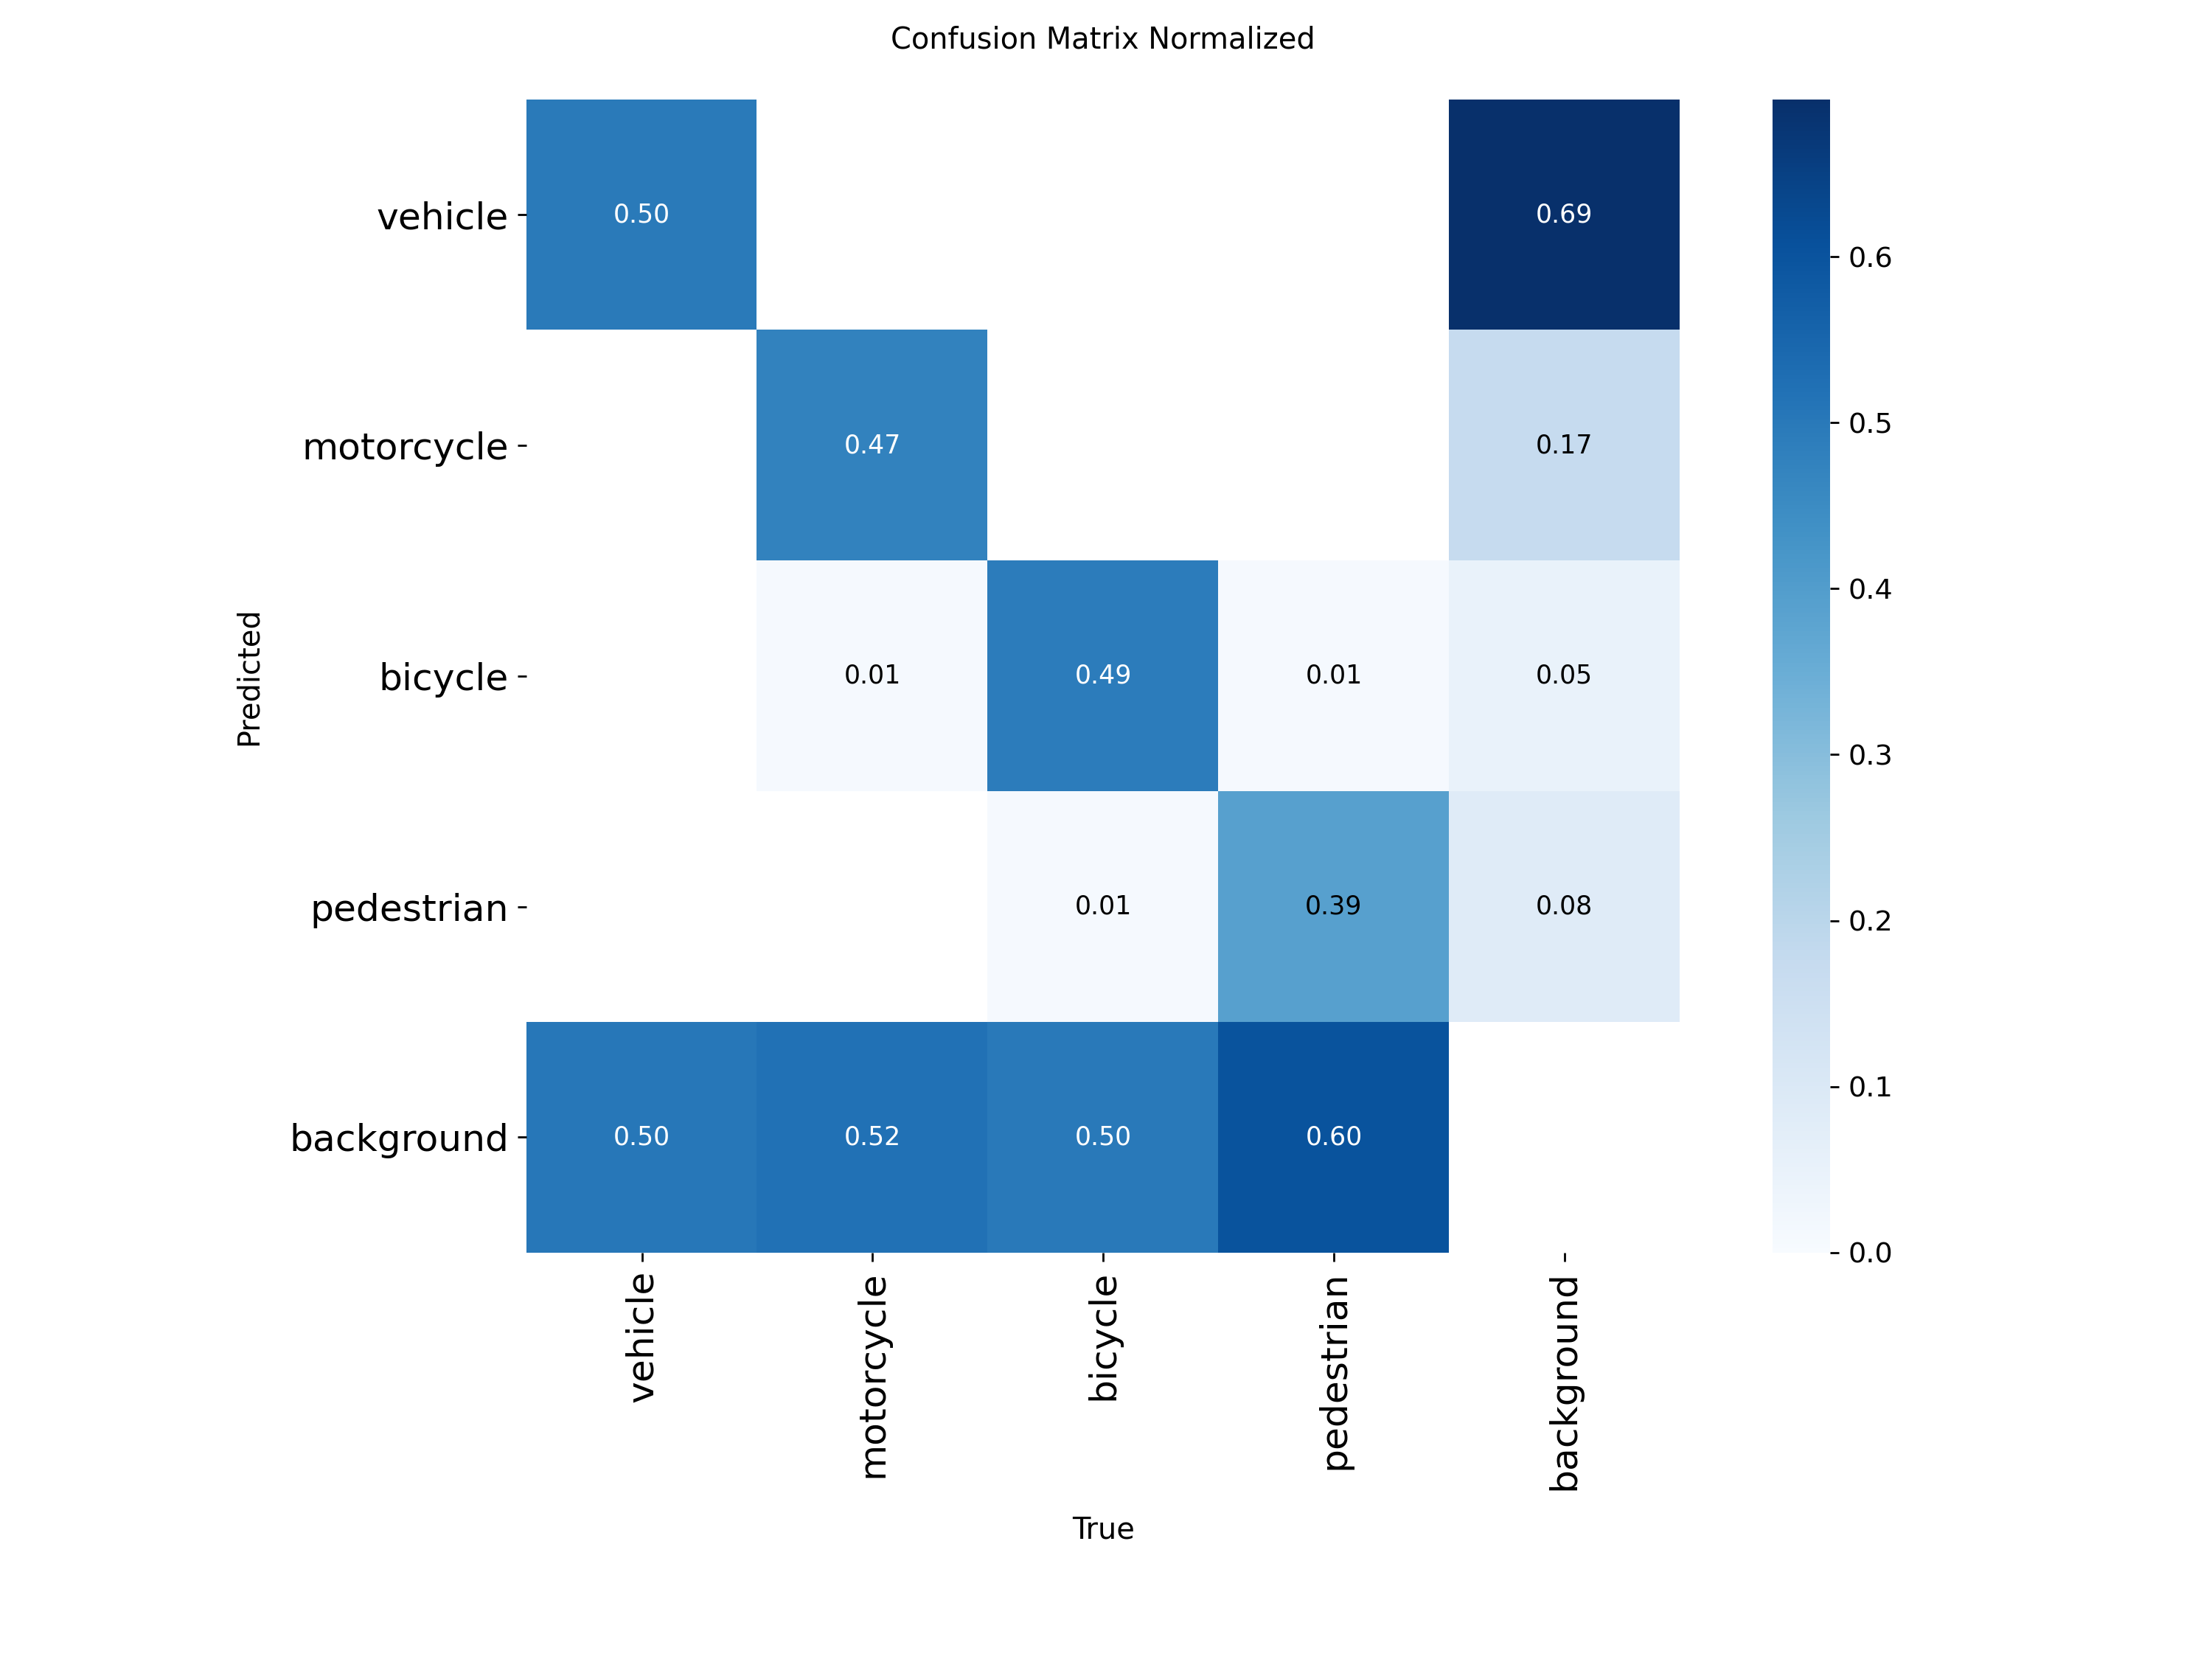
\includegraphics[width=0.62\textwidth]{fig15-detector-confusion-town10.png}
  \caption{Normalized cross-town (Town10HD) confusion matrix for the YOLO26s
  detector. Residual error concentrates among the visually similar two-wheeler
  classes and background misses.}
  \label{fig:cm}
\end{figure}

\subsection{Headline: a monotonic safety law}
The central finding is shown in Figure~\ref{fig:headline} and
Table~\ref{tab:headline}. Mean collisions per cell fall monotonically with CAV
penetration on \emph{every} arm: from the $\sim$22 all-human baseline to $\sim$6 at
full penetration, a \textbf{$\sim$73\% reduction}, with no inversion or
plateau-then-rise. Primary collisions fall in lockstep ($16.1\rightarrow5.0$ on the
Combined arm). Figure~\ref{fig:reduction} summarizes the reduction relative to the
all-human baseline: $33\%$ at $p{=}0.5$, $67\%$ at $p{=}0.9$, and $73\%$ at
$p{=}1.0$ on the Combined arm. Because reckless human drivers are progressively
replaced by cooperative AVs that brake on infrastructure- and peer-reported
hazards, the dangerous baseline is dismantled steadily rather than catastrophically.

\begin{figure}[t]
  \centering
  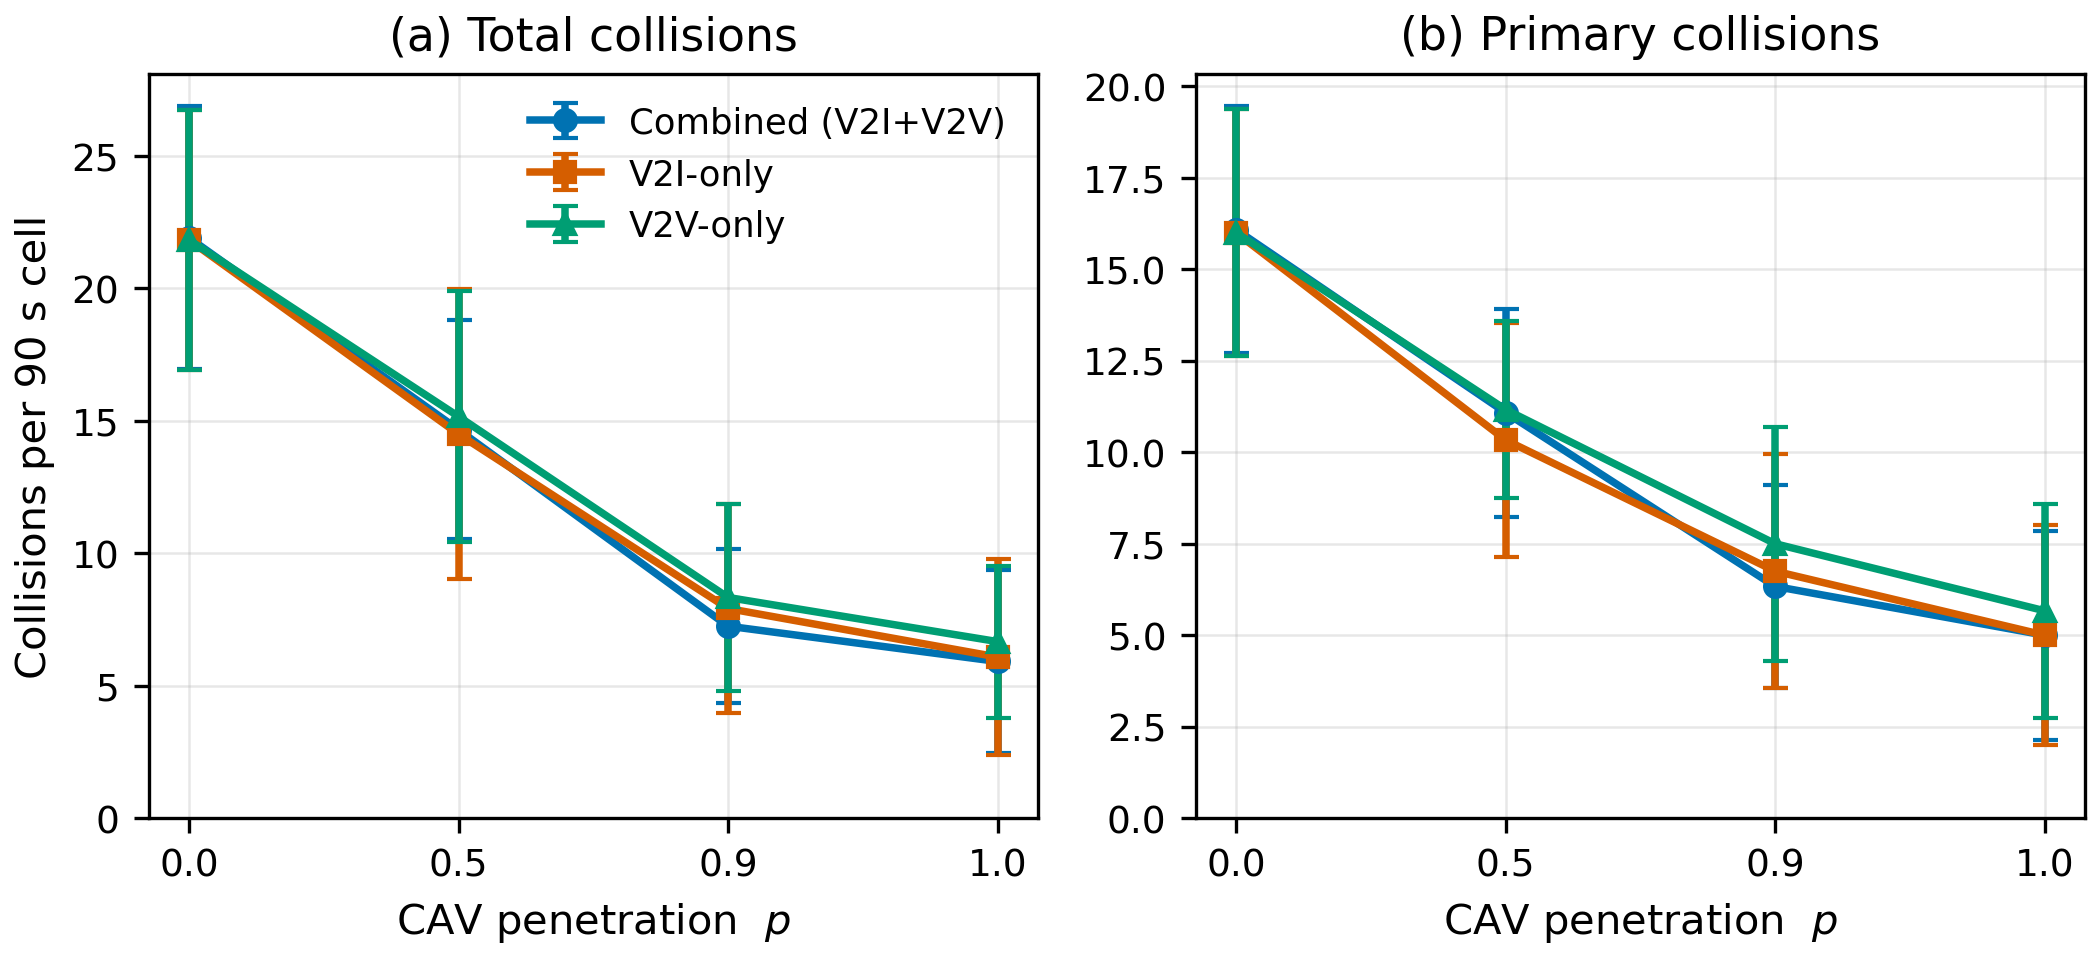
\includegraphics[width=\textwidth]{fig03-collisions-vs-penetration.png}
  \caption{Total (a) and primary (b) collisions per 90\,s cell vs.\ CAV
  penetration for the three communication arms. Error bars are $\pm1$\,SD over the
  12 cells per point. The decline is monotonic on every arm.}
  \label{fig:headline}
\end{figure}

\begin{figure}[t]
  \centering
  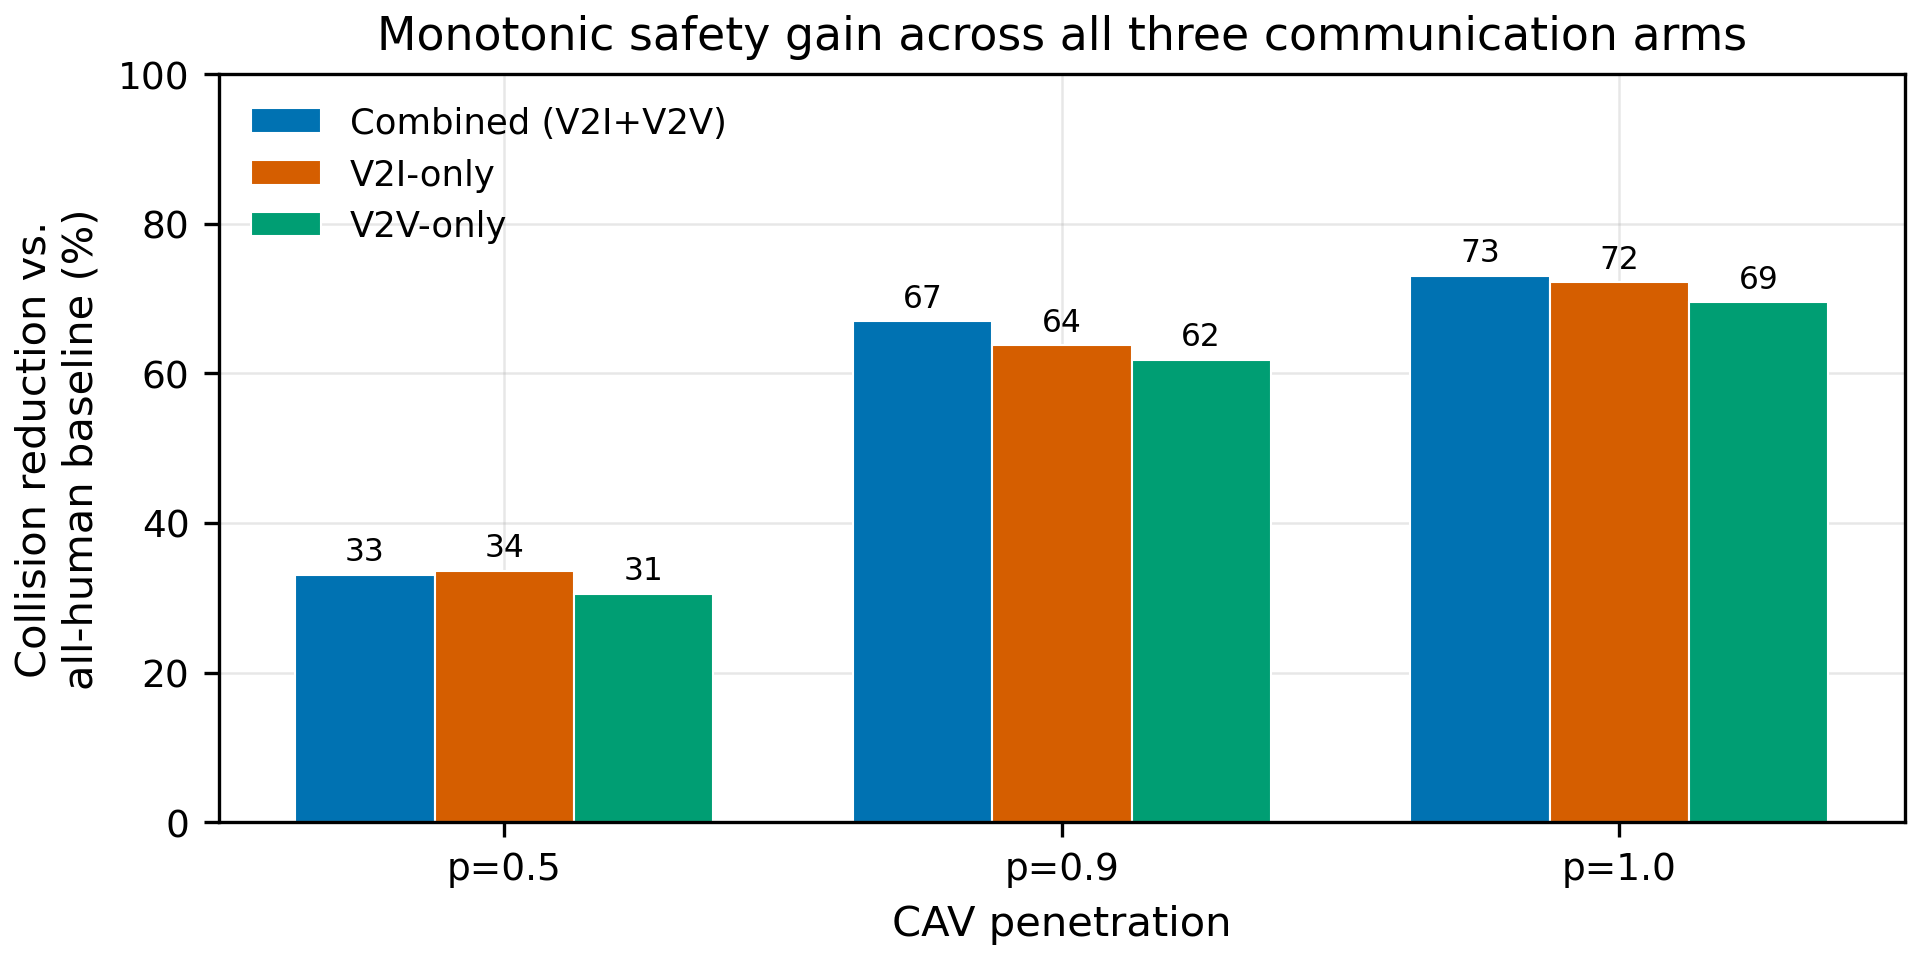
\includegraphics[width=0.84\textwidth]{fig-reduction-summary.png}
  \caption{Collision reduction relative to the all-human baseline. The gain is
  monotonic in penetration and consistently ordered Combined $\geq$ V2I-only
  $\geq$ V2V-only.}
  \label{fig:reduction}
\end{figure}

\begin{table}[t]
  \centering
  \caption{Total collisions per cell (mean\,$\pm$\,SD over 12 cells) and reduction
  vs.\ the $p{=}0$ baseline.}
  \label{tab:headline}
  \small
  \begin{tabular}{ccccc}
    \toprule
    $p$ & Combined & V2I-only & V2V-only & Reduction (Comb.) \\
    \midrule
    0.0 & $21.9\pm5.0$ & $21.8\pm4.9$ & $21.8\pm4.9$ & --- \\
    0.5 & $14.7\pm4.1$ & $14.5\pm5.5$ & $15.2\pm4.7$ & $33\%$ \\
    0.9 & $7.2\pm2.9$  & $7.9\pm3.9$  & $8.3\pm3.5$  & $67\%$ \\
    1.0 & $5.9\pm3.5$  & $6.1\pm3.7$  & $6.7\pm2.9$  & $73\%$ \\
    \bottomrule
  \end{tabular}
\end{table}

\subsection{Communication-arm ordering: infrastructure dominates}
A consistent, mild ordering holds at every penetration:
\textbf{Combined $\leq$ V2I-only $\leq$ V2V-only}. Infrastructure CPM is the
stronger single channel: the elevated, fixed RSU vantage observes the occluded
conflict zones directly and reaches all in-range CAVs, whereas V2V coverage is
contingent on a suitably placed equipped peer and a shorter $150$\,m range.
V2V-only is the weakest arm yet still cuts collisions by $\sim$69\% at full
penetration, and combining both channels is best. The gap is small relative to the
cell-to-cell standard deviation, so we report it as a robust ordering rather than a
strong separation---consistent with the two-seed design (Section~\ref{sec:threats}).

\subsection{Collision burden redistributes from humans to the fleet}
Figure~\ref{fig:who} decomposes Combined-arm collisions by party. At the baseline,
essentially all $\sim$22 collisions involve HDVs; as penetration rises, HDV-involved
collisions vanish ($21.9\rightarrow0$) while the small residual is CAV-involved
($0\rightarrow5.9$)---necessarily so, since at $p{=}1.0$ every vehicle is a CAV.
The absolute count nonetheless falls sharply, so the cooperative fleet does not
merely \emph{reallocate} risk; it removes most of it. Immobilized (``frozen'')
vehicles fall in step, from $36.4$ to $10.2$ per cell.

\begin{figure}[t]
  \centering
  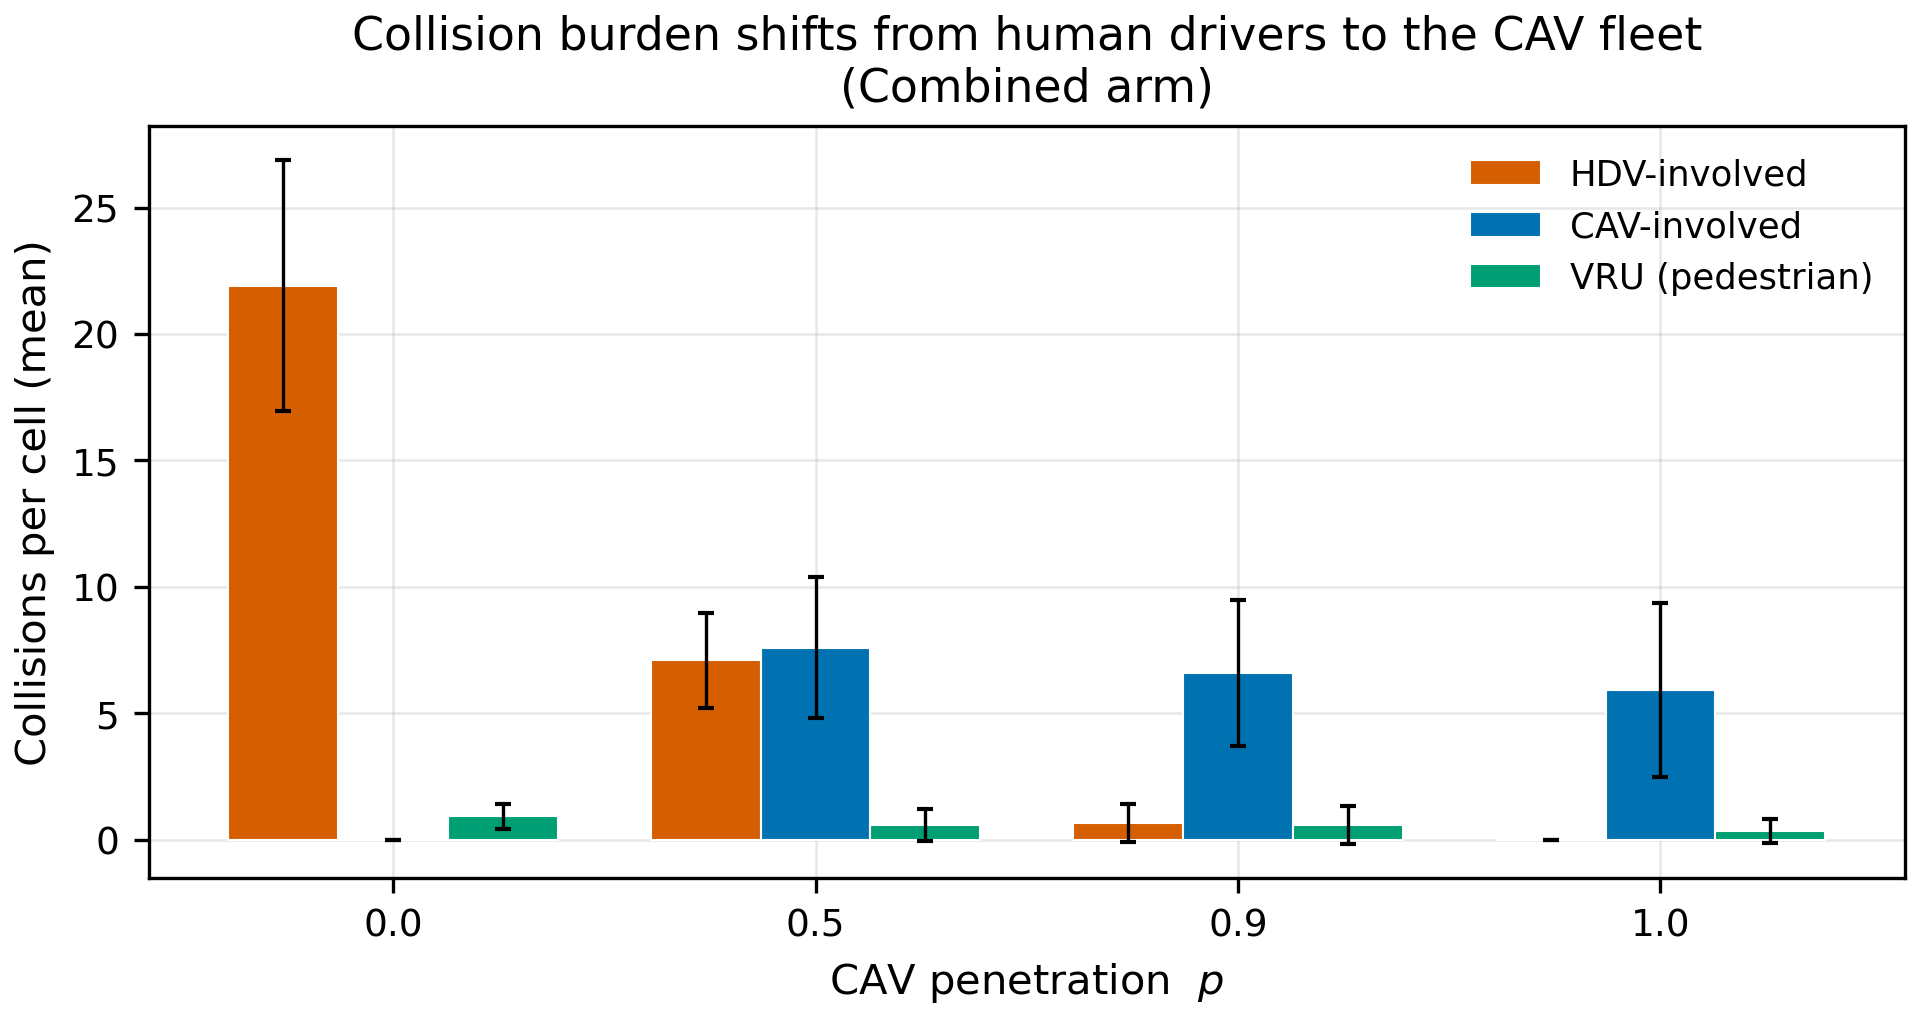
\includegraphics[width=0.82\textwidth]{fig04-who-crashes.png}
  \caption{Collisions by involved party vs.\ penetration (Combined arm). The
  burden shifts off human drivers as the dangerous baseline is dismantled.}
  \label{fig:who}
\end{figure}

\subsection{Map complexity sets the collision floor}
Figure~\ref{fig:map} stratifies by map. Town05 (multi-lane) is cleanest, with
collisions nearly eliminated ($\sim$1.8) at full penetration; Town01 (grid) drops
to $\sim$6; Town10HD (dense downtown) is hardest and plateaus around $\sim$10. The
downtown plateau is partly attributable to CARLA Traffic-Manager wide-turn
artifacts at tight, complex junctions---geometric conflicts the cooperative layer
cannot fully prevent---so this map caps the headline average rather than reflecting
a cooperative-perception failure.

\begin{figure}[t]
  \centering
  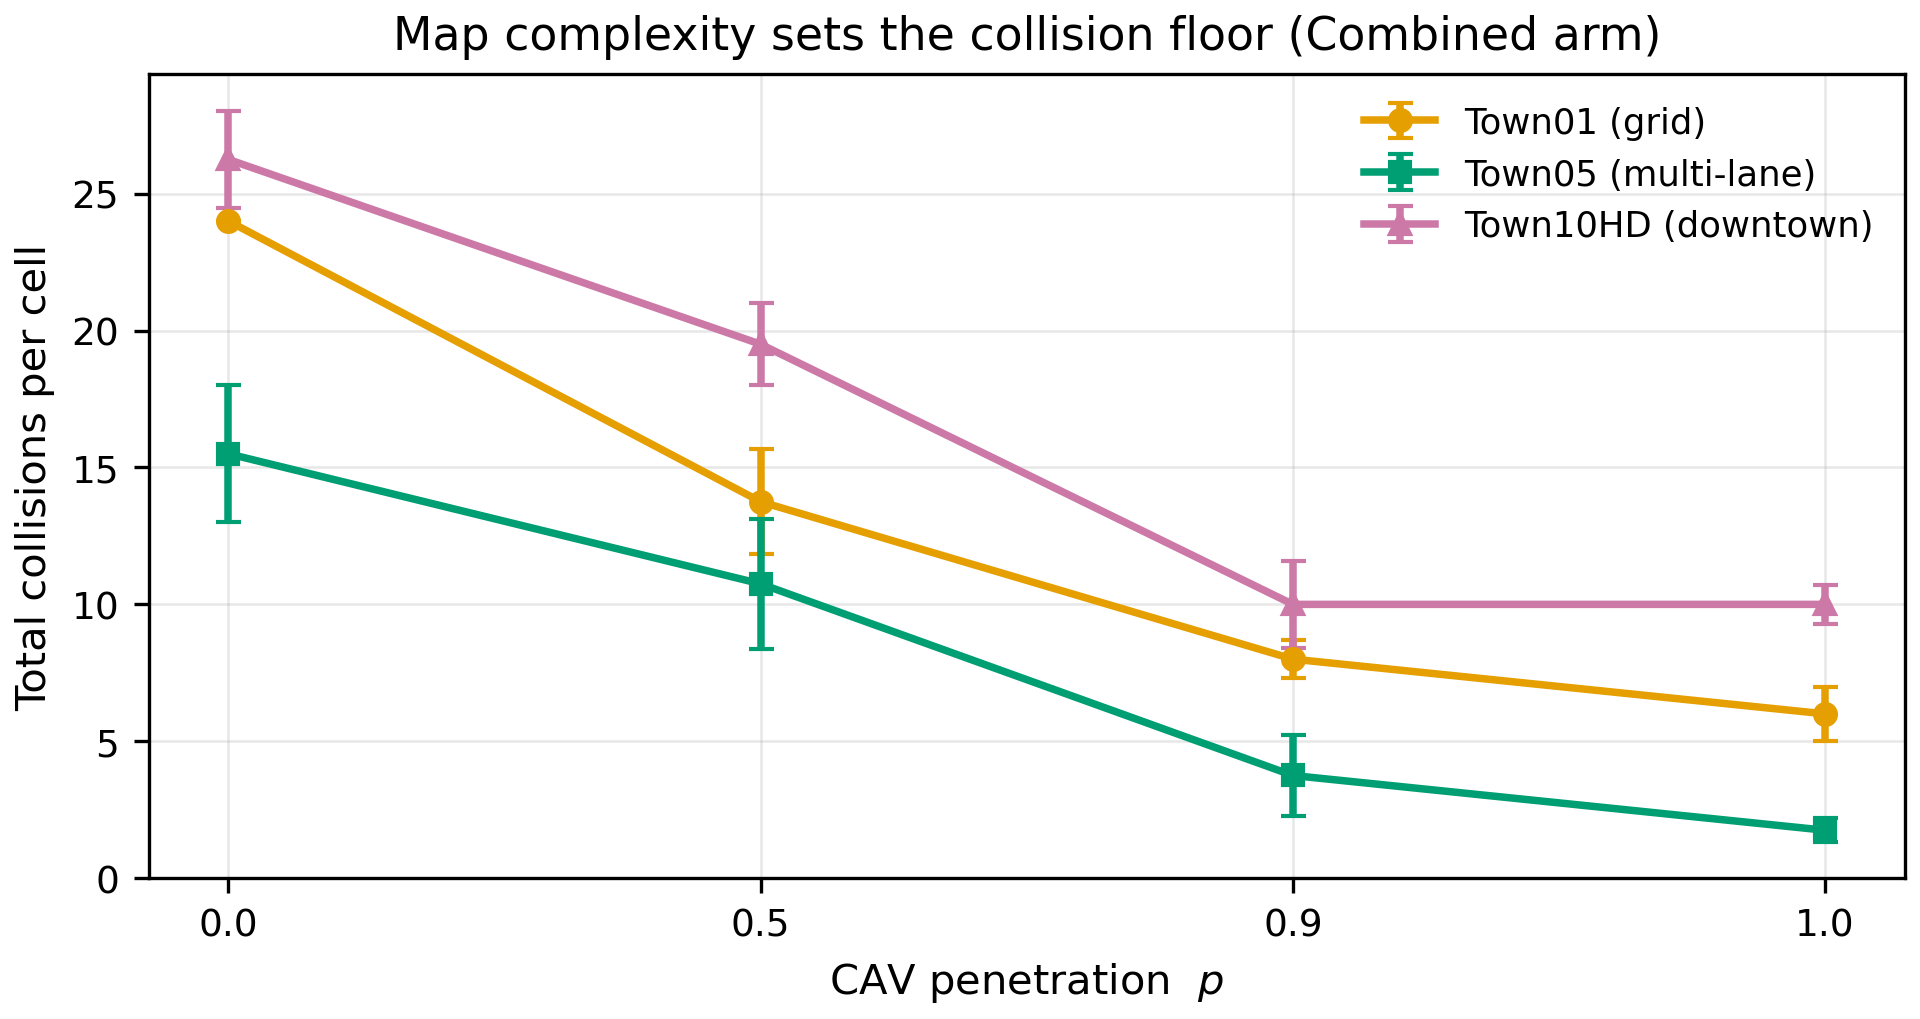
\includegraphics[width=0.82\textwidth]{fig05-collisions-by-map.png}
  \caption{Total collisions vs.\ penetration by map (Combined arm). Map complexity
  sets the achievable floor.}
  \label{fig:map}
\end{figure}

\subsection{Weather robustness}
Figure~\ref{fig:weather} compares ClearNoon and HardRainNoon on the Combined arm.
The two curves track each other closely at every penetration; the cooperative
stack is robust to the heavy-rain preset. (We note that this sweep deliberately
excludes the low-sun ClearSunset preset, whose adverse interaction is analyzed
separately in Section~\ref{sec:additional}.)

\begin{figure}[t]
  \centering
  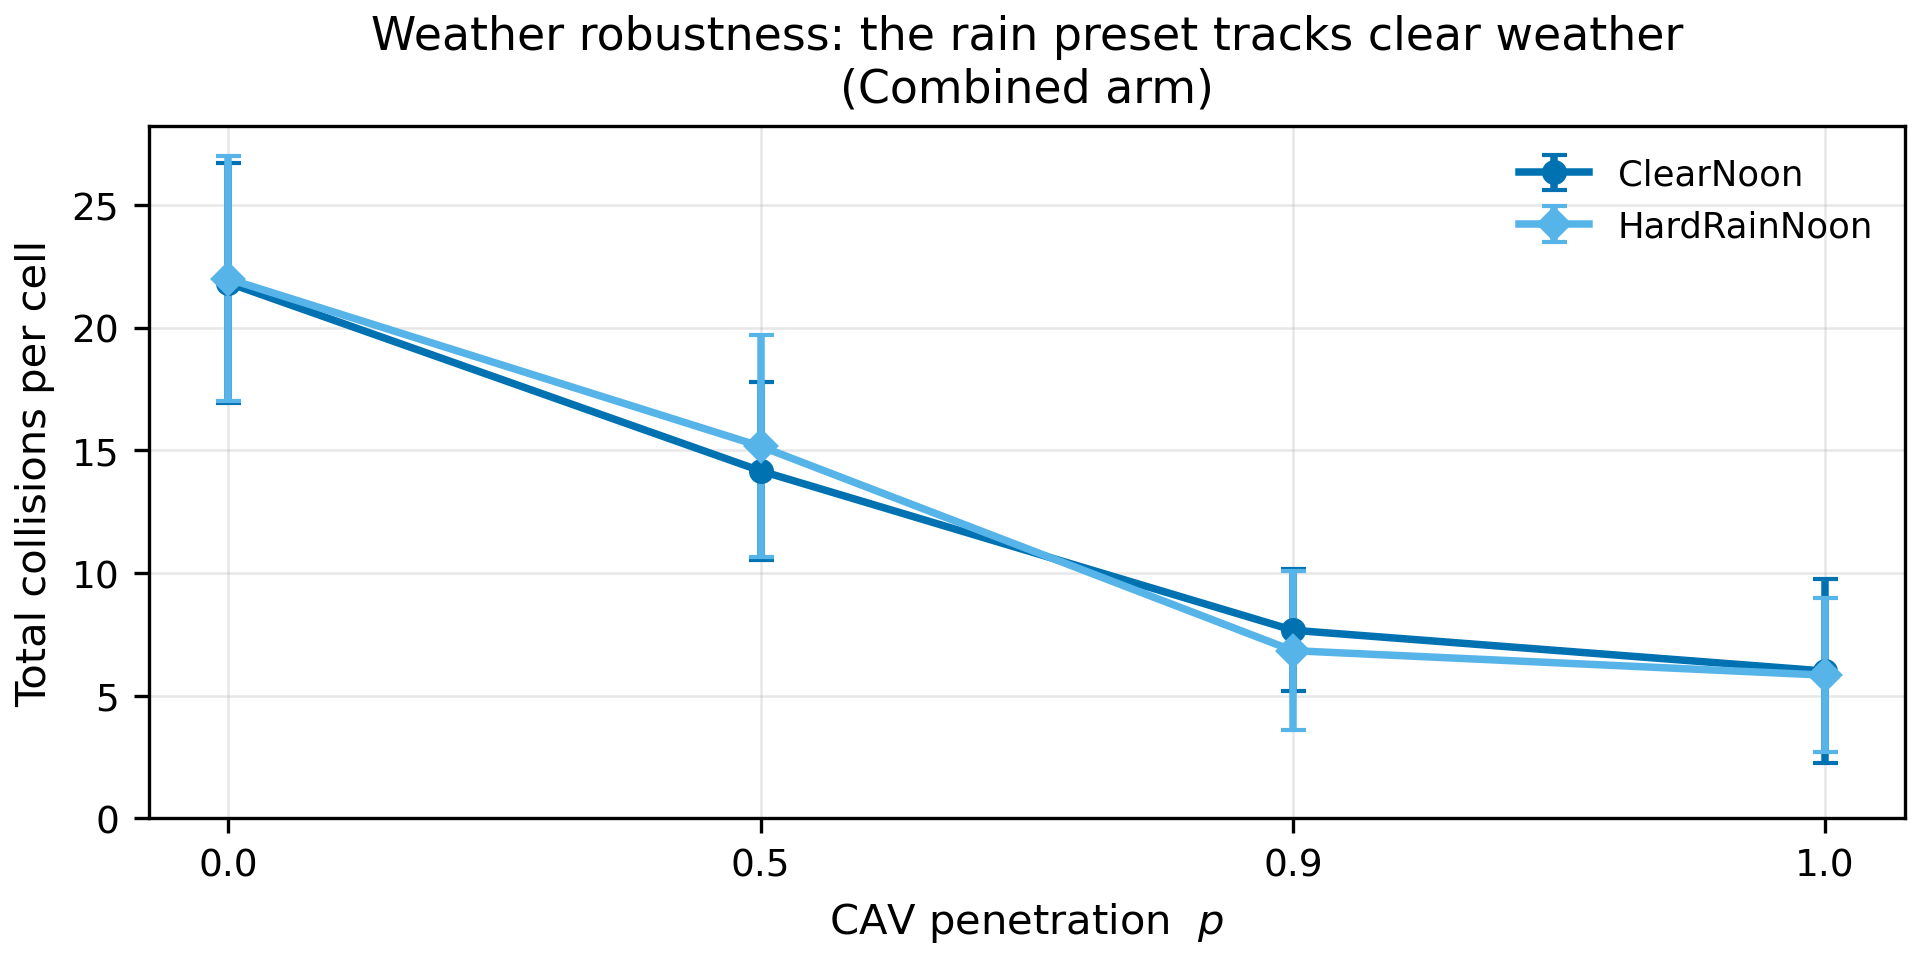
\includegraphics[width=0.78\textwidth]{fig06-collisions-by-weather.png}
  \caption{Total collisions vs.\ penetration by weather (Combined arm). Heavy rain
  tracks clear weather.}
  \label{fig:weather}
\end{figure}

\subsection{Mechanism: evasive actions, channel load, and phantom suppression}
Three internal signals confirm that the safety gain is produced by the cooperative
mechanism rather than an artifact. First, CAV evasive actions scale with
penetration (Figure~\ref{fig:actions}); the wide $7$\,m CAV headway shifts braking
away from panic hard stops toward graded soft braking and deceleration. Second,
cooperative-communication load scales as expected (Figure~\ref{fig:coop}): on the
Combined arm, delivered V2V messages rise to $\sim$0.8\,M per cell and
V2V-triggered cooperative brakes to $\sim$707. This raises the measured
channel-busy ratio with V2V volume to $\sim$0.40 at full penetration on the
Combined arm---versus a near-constant $\sim$0.016 on V2I-only, which carries only
RSU CPMs---a moderate load that nonetheless stays below saturation, so the latency
and delivery models remain in their well-behaved regime. Infrastructure CPM thus
achieves comparable safety at a small fraction of the channel occupancy demanded by
dense V2V. Third, the confirmation-hysteresis filter suppresses an increasing
number of phantom brakes as message volume grows (Figure~\ref{fig:phantom}): from
$0$ at the baseline to $\sim$47 per cell at full penetration on the Combined arm,
and---tellingly---more on infrastructure-rich arms (Combined $>$ V2I-only $>$
V2V-only), exactly where more single, unconfirmed CPMs must be filtered.

\begin{figure}[t]
  \centering
  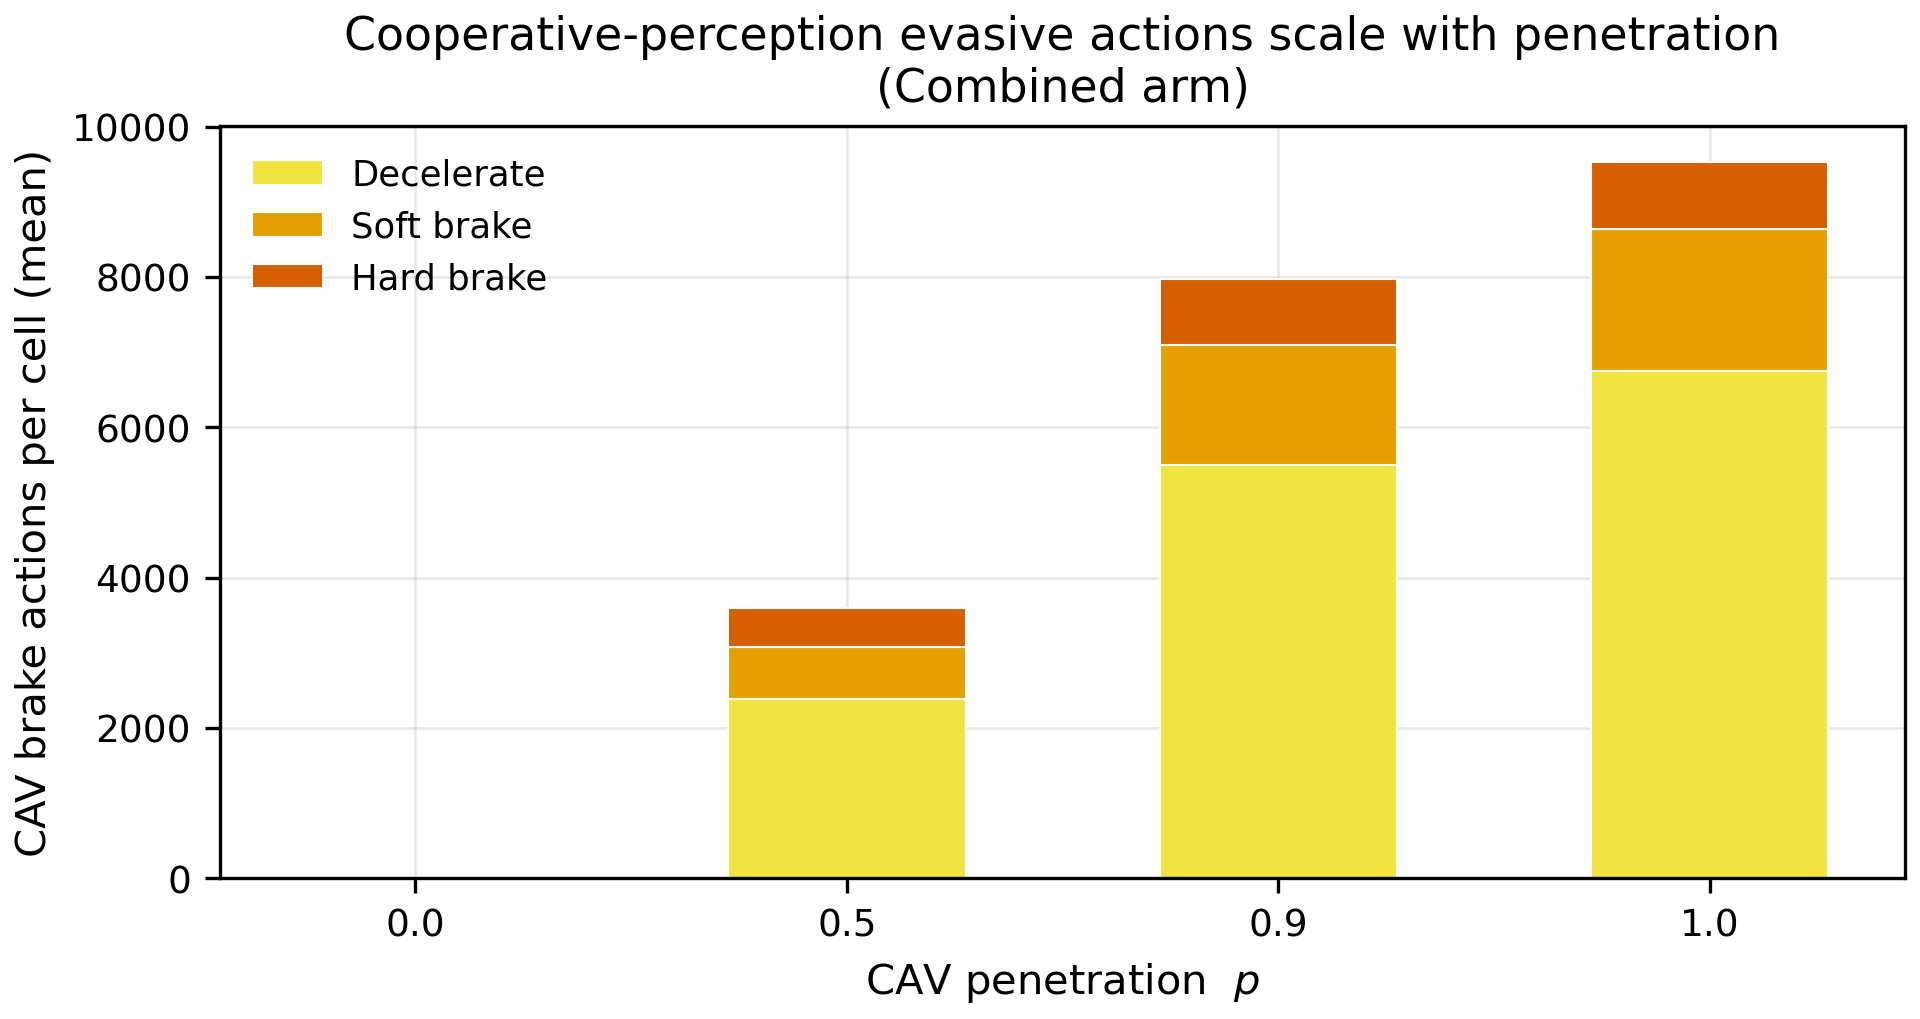
\includegraphics[width=0.80\textwidth]{fig07-brake-actions.png}
  \caption{CAV evasive brake actions vs.\ penetration (Combined arm).}
  \label{fig:actions}
\end{figure}

\begin{figure}[t]
  \centering
  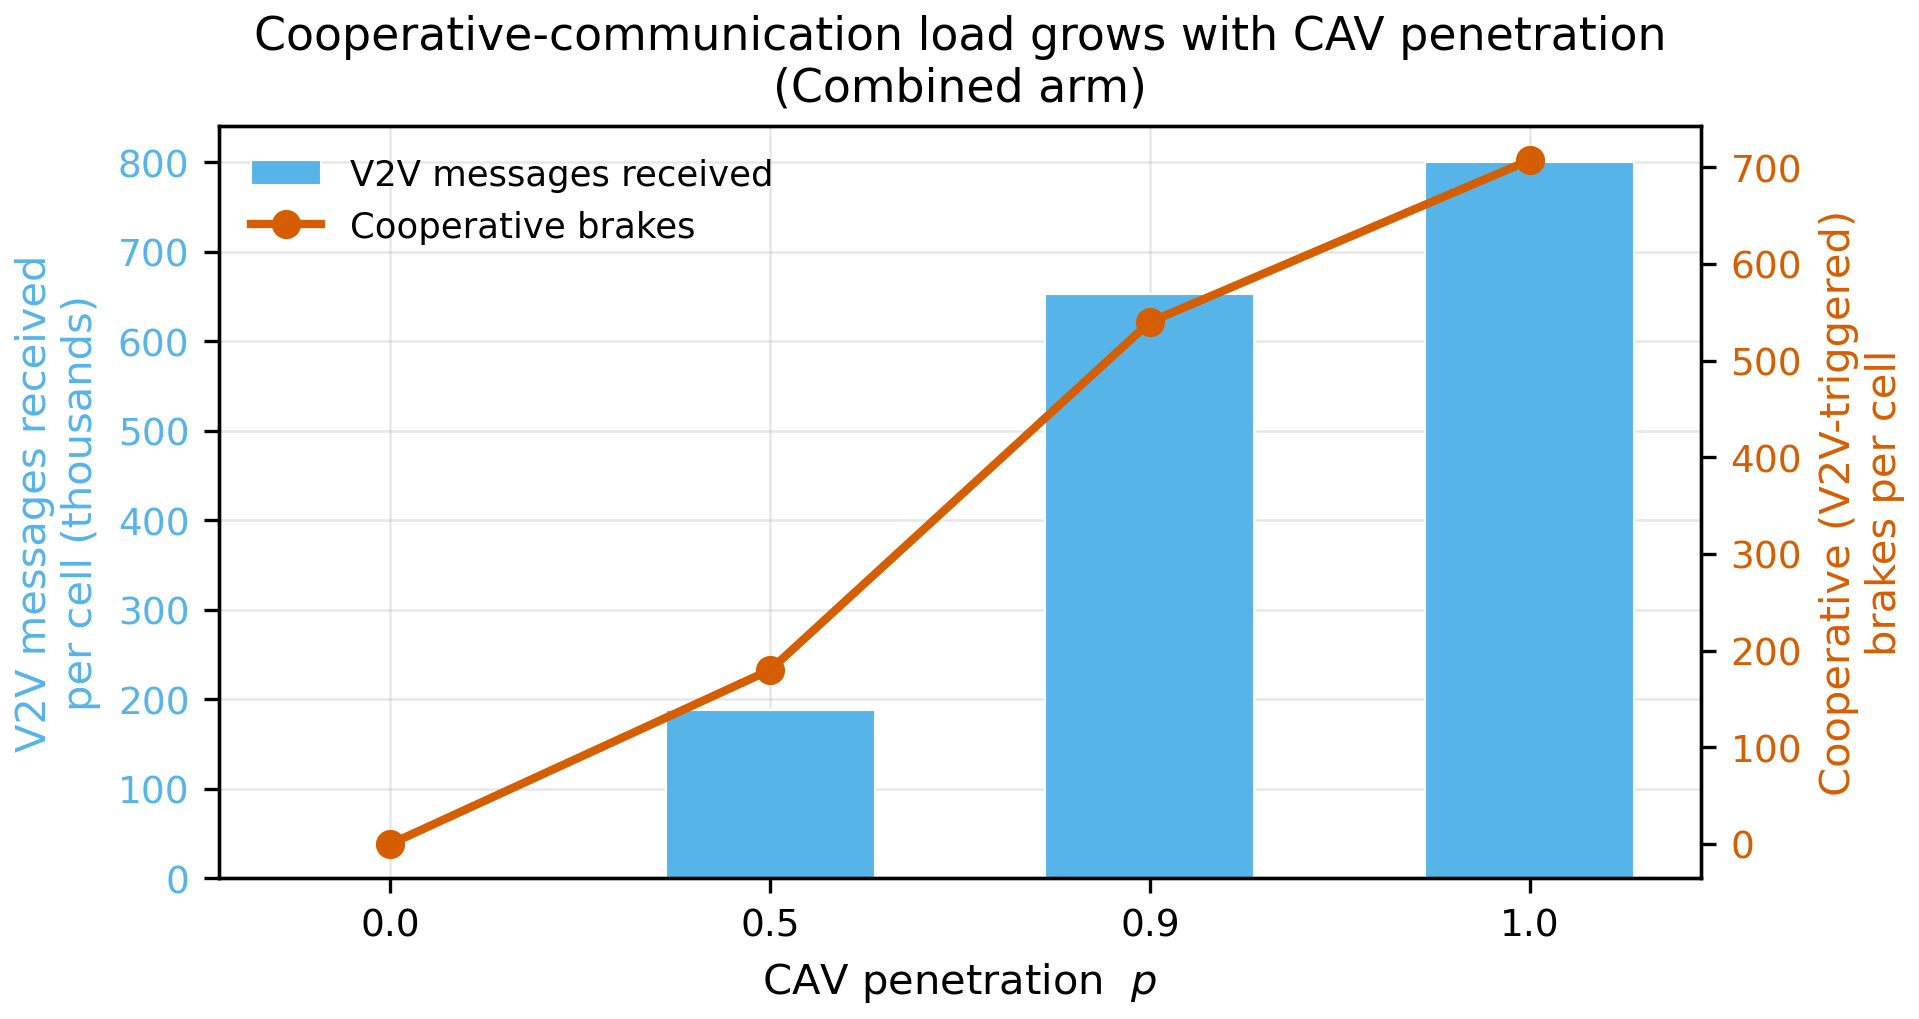
\includegraphics[width=0.80\textwidth]{fig08-coop-load.png}
  \caption{Cooperative-communication load vs.\ penetration (Combined arm):
  delivered V2V messages (bars) and V2V-triggered cooperative brakes (line).}
  \label{fig:coop}
\end{figure}

\begin{figure}[t]
  \centering
  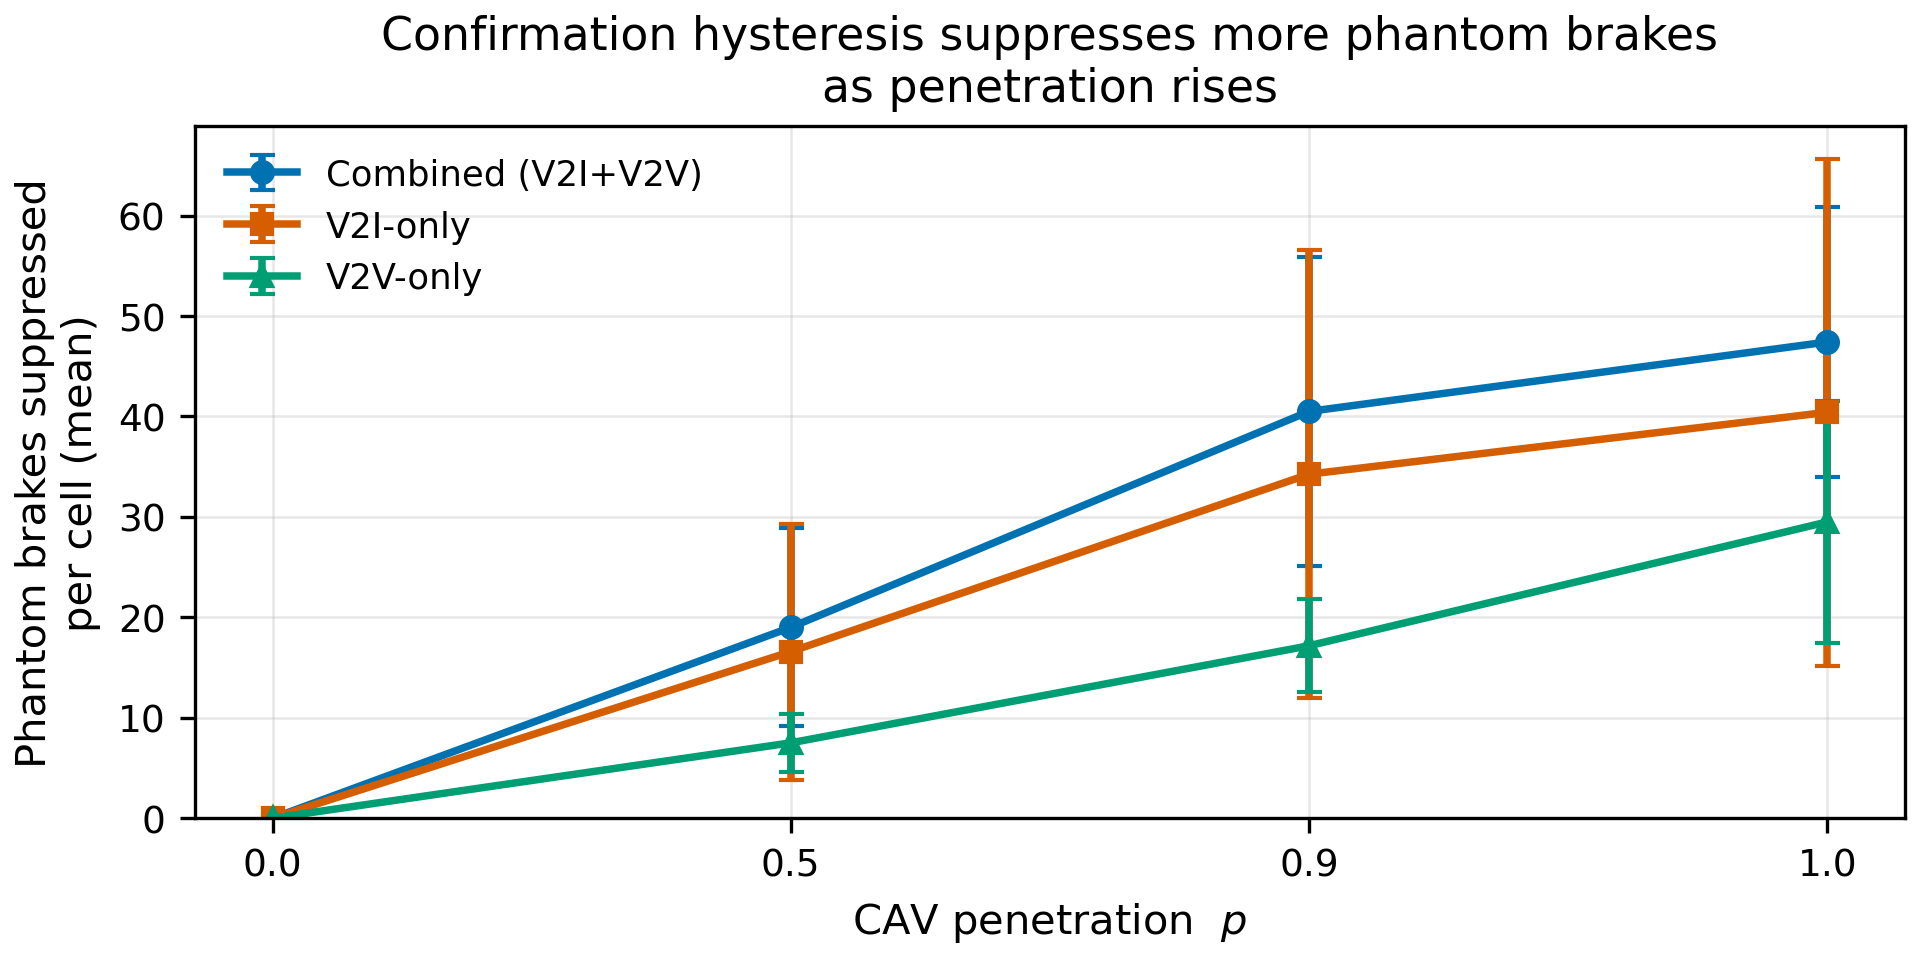
\includegraphics[width=0.78\textwidth]{fig09-phantom-brakes.png}
  \caption{Phantom brakes suppressed by the confirmation-hysteresis filter vs.\
  penetration, by arm. Suppression grows with message volume and is highest on the
  infrastructure-rich arms.}
  \label{fig:phantom}
\end{figure}

\subsection{Vulnerable road users}
Figure~\ref{fig:vru}(a) shows VRU (pedestrian) collisions vs.\ penetration: a
low-count, noisy metric that nonetheless trends downward
($\sim$0.9$\rightarrow$0.3 per cell on the Combined arm). More informative is the
\emph{redistribution} of who strikes the pedestrian
(Figure~\ref{fig:vru}(b)): HDV-on-pedestrian incidents fall toward zero as humans
leave the fleet, while the residual shifts to CAV-on-pedestrian. The protective
mechanism is the ``eye in the sky'': the RSU detects a pedestrian stepping off the
kerb behind an occluding vehicle and broadcasts the hazard before any approaching
vehicle---human or CAV---has line of sight (Figure~\ref{fig:vruscen}). With V2V, a
leading CAV can additionally relay the alert to trailing CAVs.

\begin{figure}[t]
  \centering
  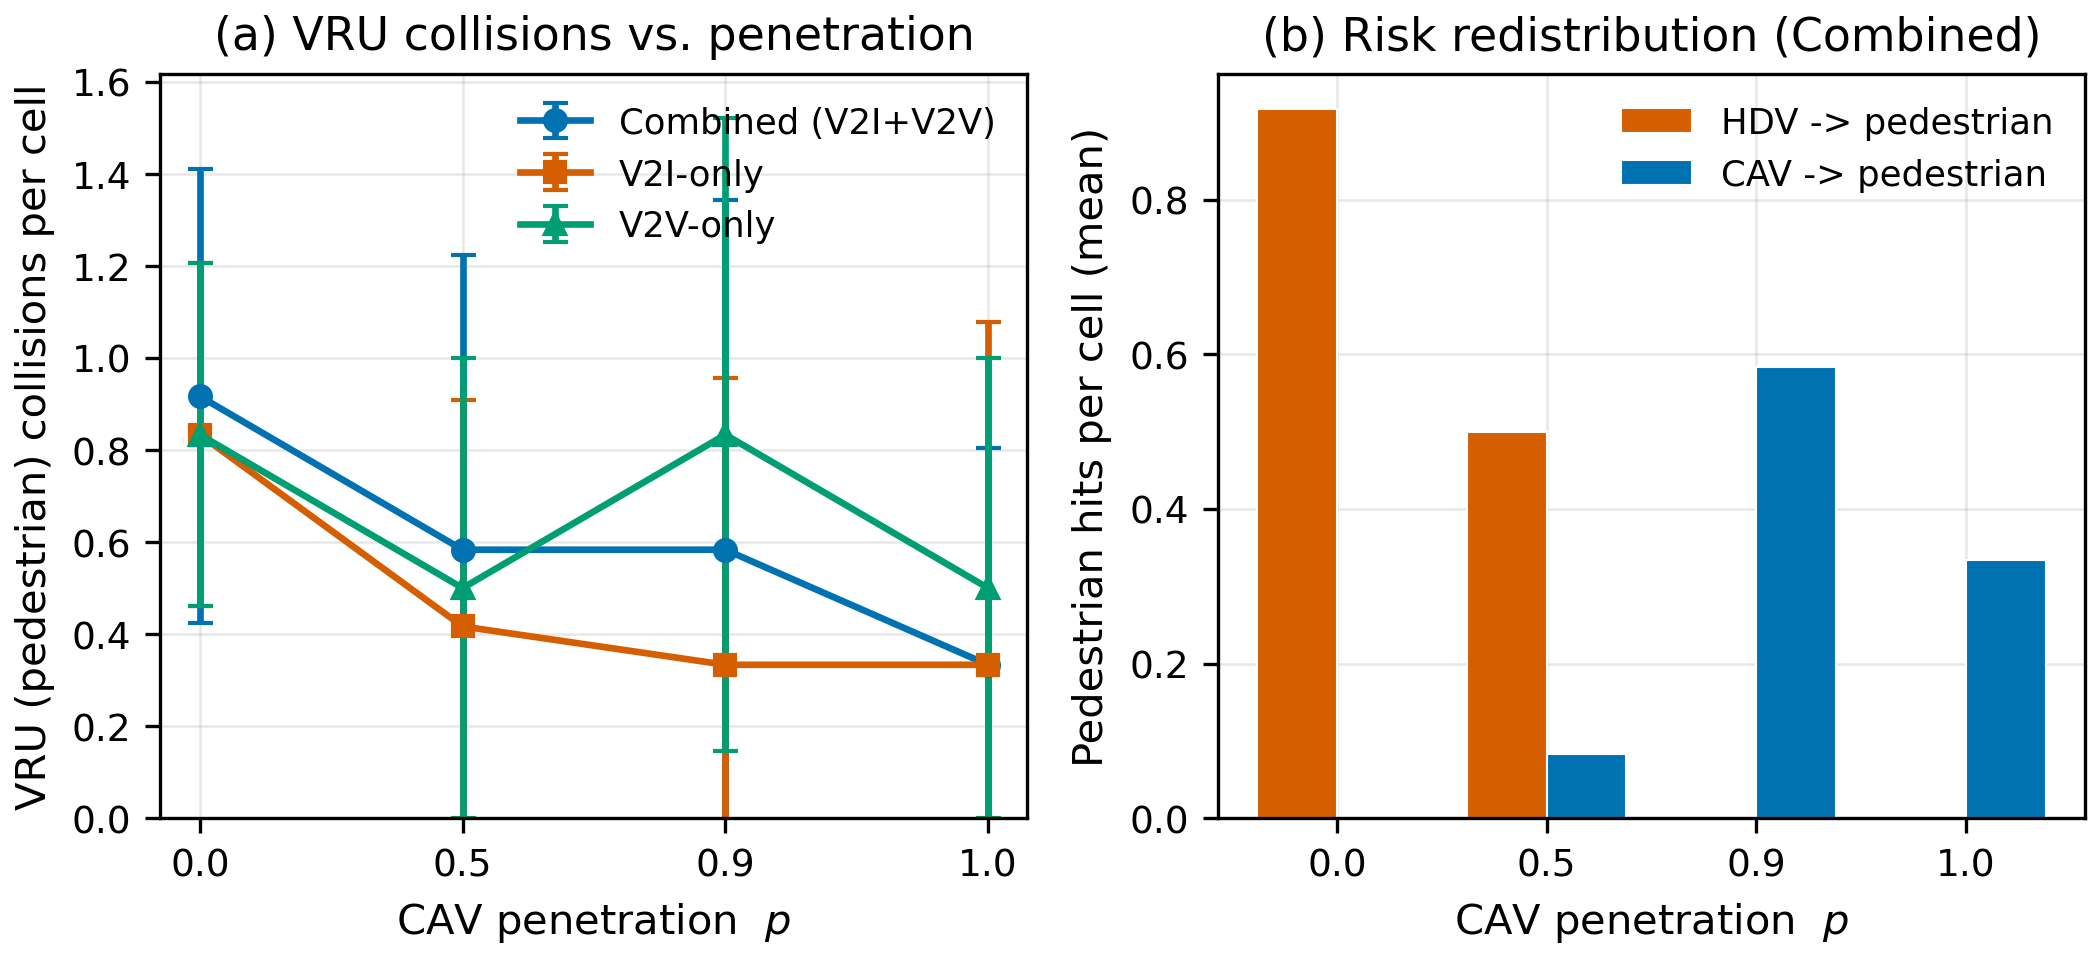
\includegraphics[width=\textwidth]{fig10-vru-collisions.png}
  \caption{(a) VRU collisions vs.\ penetration by arm. (b) Within the Combined
  arm, who strikes the pedestrian: HDV-on-VRU incidents fall toward zero while the
  small residual shifts to CAV-on-VRU.}
  \label{fig:vru}
\end{figure}

\begin{figure}[t]
  \centering
  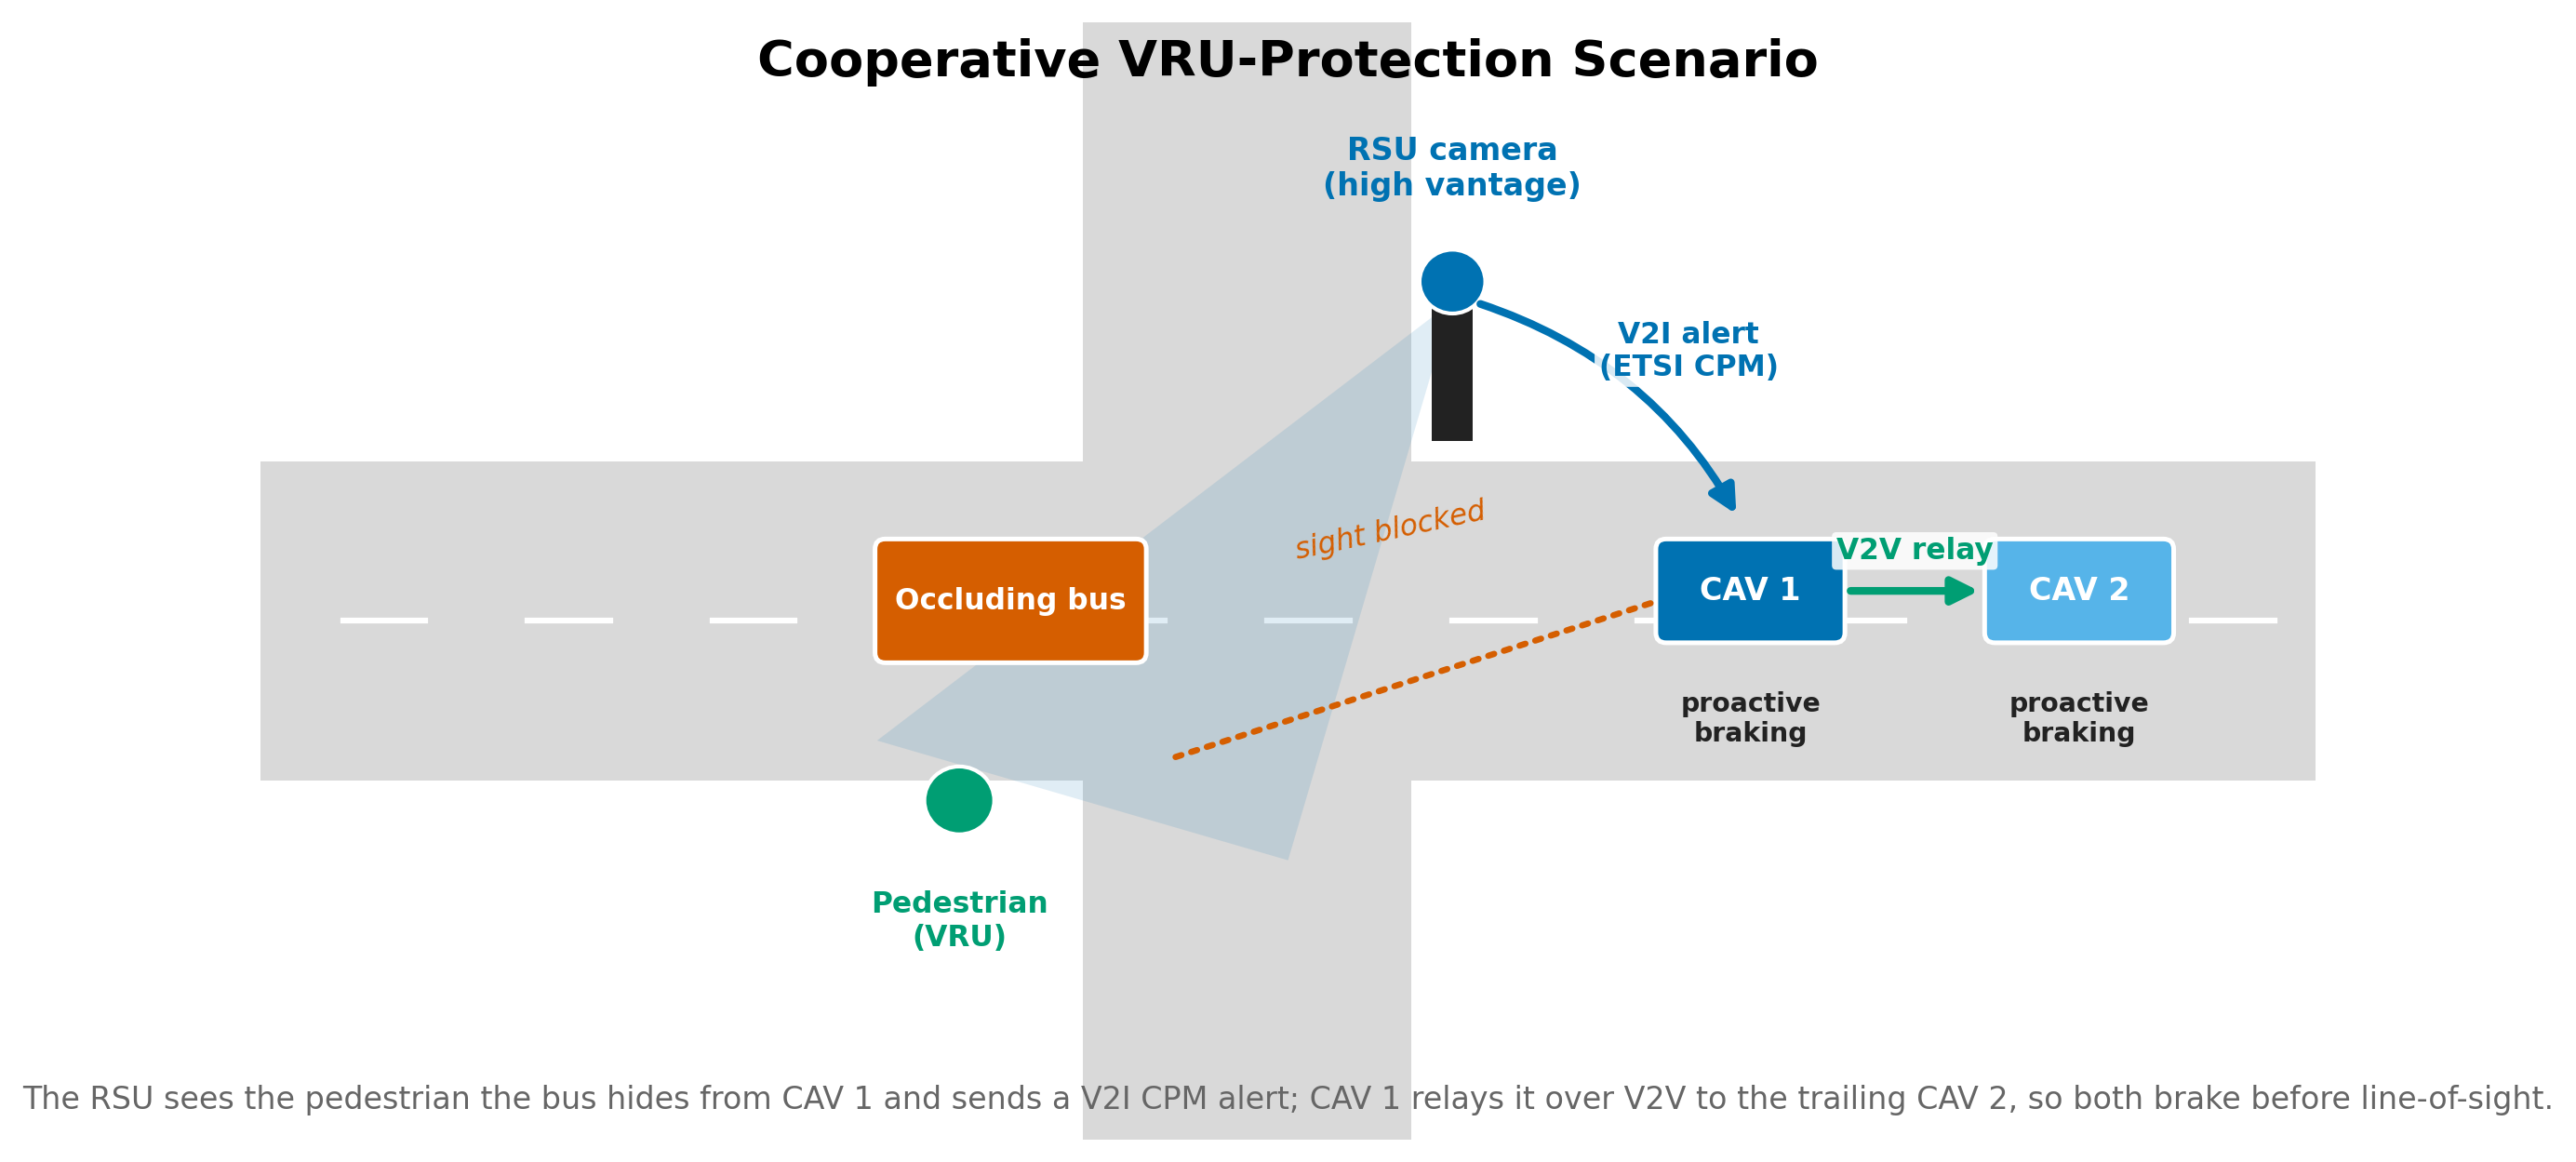
\includegraphics[width=0.86\textwidth]{fig11-vru-scenario.png}
  \caption{Cooperative VRU-protection scenario. The RSU sees the pedestrian hidden
  from CAV~1 by the bus and sends a V2I CPM alert; CAV~1 relays it over V2V to the
  trailing CAV~2, so both brake before line of sight.}
  \label{fig:vruscen}
\end{figure}

\subsection{At-fault attribution}
Figure~\ref{fig:atfault} pools at-fault collisions by driver profile across the
Combined arm. The \emph{aggressive-hostile} and \emph{distracted} profiles (both
with TM avoidance off) dominate the human-caused crashes (187 and 127), exactly as
the realism model intends, while \emph{attentive} drivers (avoidance on) appear
far less and mostly as victims. The \textsc{ai\,realistic} (CAV) count is high
(184) only because at high penetration every vehicle is a CAV, so all remaining few
collisions are necessarily CAV-involved.

\begin{figure}[t]
  \centering
  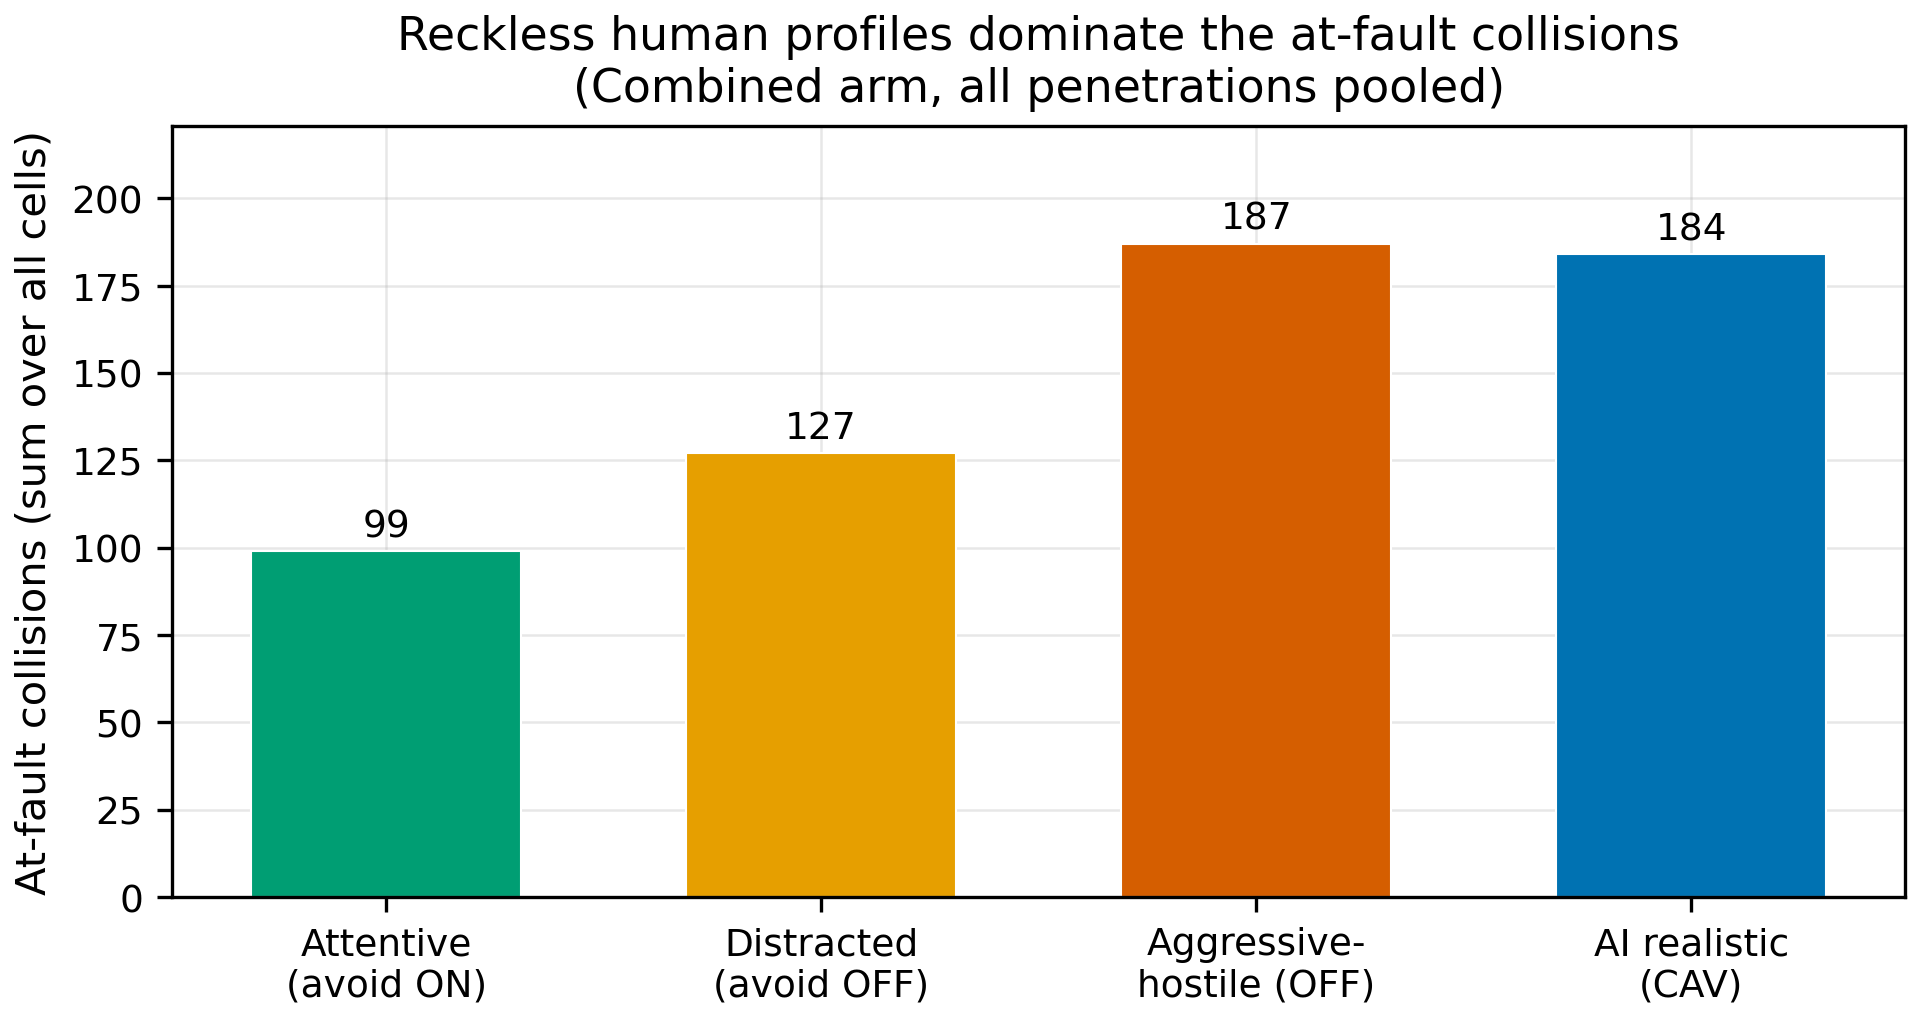
\includegraphics[width=0.80\textwidth]{fig12-atfault-by-profile.png}
  \caption{At-fault collisions by driver profile (Combined arm, all penetrations
  pooled). Reckless human profiles dominate.}
  \label{fig:atfault}
\end{figure}

% ======================================================================
\section{Framework Evolution and Earlier Sensitivity Findings}
\label{sec:additional}
% ======================================================================
The findings in this section originate from an \textbf{earlier experimental
configuration} of the framework and are retained because they probe axes the
three-arm sweep above does not. That configuration used a single always-on
cooperative path (rather than the V2I/V2V/Combined arms), penetration rates
$\{0,0.5,1.0\}$, five seeds per cell, and a different weather axis
(ClearNoon, \emph{ClearSunset}, HardRainNoon); deltas there were reported with
Welch's $t$-tests and Cohen's $d$. The headline three-arm results in
Section~5 supersede its overall-collision numbers, but the sensitivity insights
below remain instructive. The issues that motivated the framework's evolution from
that configuration to the present one are summarized in Table~\ref{tab:remediation}.

\begin{table}[t]
  \centering
  \caption{Issues identified in the earlier configuration and the remediations
  applied in the present framework. Several remediations also change how collisions
  are \emph{counted}, which is why the magnitudes in this section are not comparable
  to those in Section~5.}
  \label{tab:remediation}
  \small
  \begin{tabular}{p{0.29\linewidth} p{0.31\linewidth} p{0.32\linewidth}}
    \toprule
    Issue & Symptom & Remediation \\
    \midrule
    Overlapping spawns & Vehicles materialized inside one another, causing
      spawn-instant collisions & Minimum-separation spawn sampling ($\geq 6$\,m
      pairwise) with non-forcing \texttt{try\_spawn} \\
    Runaway collision counter & Per-contact counting inflated totals; grinding
      vehicles kept re-firing the collision sensor & One deduplicated incident per
      unordered pair, plus immobilize-in-place (brake $+$ handbrake $+$ frozen
      physics) so wrecks stop re-triggering \\
    Inverted safety curve at high penetration & Collisions \emph{rose} with CAV
      share & Velocity-matched ego self-exclusion; closing-rate gate on the distance
      fallback; $7$\,m CAV headway; steering-preserving brake override \\
    Unattributable / over-crashing HDVs & Blinding every HDV caused mass pile-ups and
      obscured fault & Role-selective avoidance: attentive keep TM avoidance;
      distracted and aggressive-hostile run with it off \\
    Non-reproducible baseline & The three arms' $p{=}0$ cells diverged & Seed the
      Traffic Manager and pedestrian-navigation RNGs from the cell seed \\
    Transient cell crashes & Occasional spawn-time server faults left gaps & Per-cell
      retry ($\times2$) and a server watchdog $\rightarrow$ 144/144 gap-free \\
    \bottomrule
  \end{tabular}
\end{table}

\noindent\textbf{A note on comparability.} The earlier configuration also
\emph{counted} collisions differently: it used a less-aggressively-deduplicated
count over $120$\,s cells, whereas the present framework counts one deduplicated
incident per vehicle pair over $90$\,s cells and immobilizes wrecks so they cannot
re-trigger the collision sensor. The two are therefore not comparable in absolute
magnitude---hence the $\sim$1180 Town05 baseline in Table~\ref{tab:old} versus the
$\sim$22 of Section~5 (the raw, undeduplicated contact-event count in the earlier
logs is larger still, $\approx$21{,}000 per cell). Consequently only the
\emph{qualitative} trends below transfer; the earlier configuration's absolute
collision counts are superseded by Section~5.

\begin{table}[t]
  \centering
  \caption{Aggregate metrics from the earlier configuration (dense 60-vehicle /
  60-walker sweep, five seeds, $120$\,s cells). Town05 totals; VRU and phantom
  counts are fleet-wide; ``$\pm$'' is population SD. These collision counts use the
  earlier deduplication and are \emph{not} comparable in magnitude to Section~5
  (see the comparability note above).}
  \label{tab:old}
  \small
  \begin{tabular}{lccc}
    \toprule
    Penetration & Total coll.\ (Town05) & VRU coll.\ (fleet) & Phantom brakes supp. \\
    \midrule
    0\% (baseline) & $1180\pm187$ & $2.07\pm2.49$ & 0 \\
    50\% (mixed)   & $1141\pm207$ & $1.82\pm1.99$ & $\sim$48 \\
    100\% (full)   & $1138\pm181$ & $1.93\pm1.64$ & $\sim$95 \\
    \bottomrule
  \end{tabular}
\end{table}

\noindent\textbf{VRU risk redistribution.} In that configuration, mean VRU
collisions stayed essentially flat overall ($\sim$2.1 per cell; see
Table~\ref{tab:old}), but the \emph{perpetrator} shifted almost one-for-one:
HDV-on-pedestrian incidents fell from $2.07$ to $0$ across penetration while
CAV-on-pedestrian rose from $0$ to $1.93$. The present three-arm data
reproduce the same qualitative redistribution (Figure~\ref{fig:vru}b).

\noindent\textbf{Traffic-density saturation.} Under extreme density (60 vehicles
$+$ 60 walkers), overall vehicle-collision benefit on Town05 saturated to a small
residual ($\sim$3.6\%), because unavoidable downstream chain reactions can overwhelm
the safety layer at gridlock. The cleaner monotonic curve in Section~5 reflects the
revised driver model, the steering-preserving brake override, and the
primary/secondary collision split, which together remove much of that saturation.

\noindent\textbf{Cross-map detector bottleneck.} Zero-shot evaluation on maps the
detector never trained on collapsed the V2X benefit toward zero, because a detector
that fails to generalize transmits noise rather than hazards. This is the operational
consequence of the 0.22 mAP cross-town gap in Table~\ref{tab:detector} and explains
why Town10HD sets a higher collision floor.

\noindent\textbf{The ClearSunset paradox.} Most counter-intuitively, under low-sun
ClearSunset glare, increasing penetration \emph{increased} collisions by
$\sim$7.7\% on Town05---the map where the effect is sharpest, with the all-map mean
rise being $\sim$3.3\%: severe glare spiked false-positive detections, and these
``ghost hazards''
propagated through the CPM stream and triggered phantom hard brakes, causing
trailing vehicles to rear-end the braking CAVs. This shows that environmental
robustness is not merely an accuracy concern but a safety constraint, and motivates
the high-precision detector operating point.

% ======================================================================
\section{Threats to Validity}
\label{sec:threats}
% ======================================================================
\begin{itemize}[leftmargin=1.3em,itemsep=0.15em,topsep=0.2em]
  \item \textbf{Seed count.} Two seeds give real but modest variance (reported as
  $\pm$SD). A larger seed count would tighten the arm-ordering confidence, which is
  small relative to the cell-to-cell SD.
  \item \textbf{Immobilize-in-place.} Crashed vehicles are frozen in place, which
  can couple incidents; the primary/secondary split mitigates this, and we report
  the primary metric alongside the total.
  \item \textbf{Junction geometry.} A fraction of Town10HD high-penetration
  collisions are CARLA Traffic-Manager wide-turn artifacts rather than genuine
  cooperative-perception failures, inflating that map's floor.
  \item \textbf{Channel abstraction.} The 5G~NR-V2X channel is parametric
  (Coll-Perales/Thandavarayan), not a full-stack ns-3/5G-LENA simulation; results
  should be read as relative, not absolute.
  \item \textbf{Synthetic-to-real gap.} All perception and physics are simulated;
  the contribution is the \emph{relative} safety law across penetration and arms,
  not absolute collision counts.
  \item \textbf{Idealized CAV localization.} CAVs receive near-ground-truth ego
  pose and a clean local-sensor cone, so the measured benefit is an optimistic
  upper bound rather than a deployment estimate.
\end{itemize}

% ======================================================================
\section{Future Directions}
% ======================================================================
Direct V2V relaying, identified as future work in the earlier V2I-only study, is
realized here; the remaining directions are:
\begin{itemize}[leftmargin=1.3em,itemsep=0.15em,topsep=0.2em]
  \item \textbf{Full-stack channel.} Replace the parametric channel with an
  ns-3/5G-LENA sidelink stack to cross-validate the latency/PDR assumptions and
  model congestion at higher densities.
  \item \textbf{Network visualization.} A live, in-UI overlay of per-CPM flows,
  per-link latency, CBR over time, and PDR drops (the demonstration application in
  Appendix~\ref{app:demo} is a first step).
  \item \textbf{Deployable OBU.} Package the CAV cooperative core into an
  integratable on-board unit (MQTT over 5G) so legacy vehicles can receive HUD
  warnings, extending the benefit beyond fully autonomous fleets.
\end{itemize}

% ======================================================================
\section{Conclusion}
% ======================================================================
We presented V2X-Sim, an end-to-end cooperative-perception framework in CARLA that
couples an empirical YOLO26s pipeline, ETSI CPM Release~2 payloads, and realistic
5G~NR-V2X channel and edge-compute models, and extended it to support V2I, V2V, and
combined communication. A 144-cell, three-arm penetration ablation in dense hostile
traffic yields a clean, monotonic safety law---a $\sim$73\% collision reduction from
the all-human baseline to a fully cooperative fleet---robust across maps and
weather, with infrastructure CPM identified as the dominant single channel
(Combined $\leq$ V2I-only $\leq$ V2V-only). Map complexity, not weather, sets the
collision floor, and the cooperative mechanism is corroborated by graded evasive
actions, scaling cooperative-communication load at low channel occupancy, and
growing phantom-brake suppression. Together with the retained sensitivity findings,
the study argues that cooperative perception delivers a substantial, attributable
safety benefit---bounded chiefly by detector generalization and simulator junction
geometry rather than by the communication channel itself.

% ----------------------------------------------------------------------
\bibliographystyle{IEEEtran}
\bibliography{references}

% ======================================================================
\appendix
\section{Interactive Demonstration Application}
\label{app:demo}
% ======================================================================
To make the otherwise-invisible V2X pipeline observable, the framework ships an
interactive demonstration application (\texttt{51\_demo\_ui.py}) built with
\textsc{DearPyGui}. It presents a single-window, four-panel dashboard
(Figures~\ref{fig:ui1}--\ref{fig:ui3}) and auto-minimizes CARLA's native window so
that everything the user needs sits in one viewport; it supersedes an earlier
multi-window visualizer.

\noindent\textbf{Panels.}
\begin{itemize}[leftmargin=1.3em,itemsep=0.15em,topsep=0.2em]
  \item \textbf{Configuration} (top-left): a map selector, weather selector,
  per-RSU intersection check-boxes, and sliders for the number of vehicles, CAV
  penetration (\%), number of pedestrians, and simulation duration, with
  \textsc{start}/\textsc{stop} controls and a running-status line. Maps can be
  switched live from the UI.
  \item \textbf{CARLA Bird's-eye View} (top-right): a live top-down render of the
  scene overlaid with RSU positions and the active V2X communication links and
  coverage rays.
  \item \textbf{Live Statistics} (bottom-left): real-time telemetry including
  map/weather, simulation time, wall time and wall-to-sim ratio, number of
  signalized intersections, broadcast range, active CPM links, RSU detection links,
  total CPMs transmitted, the count of V2X-equipped CAVs, the per-profile HDV
  breakdown (attentive / distracted / aggressive), and per-tick YOLO detection
  counts.
  \item \textbf{RSU Cameras} (bottom-right): a tabbed, per-RSU $1280\times720$
  camera feed with the live YOLO26s bounding-box overlay and per-RSU statistics, so
  each infrastructure sensor can be inspected individually.
\end{itemize}

\noindent\textbf{Features.} The application provides (i) interactive scenario
configuration (map, weather, fleet composition, penetration, RSU placement);
(ii) one-click run control and live map switching; (iii) real-time detection
visualization with YOLO bounding boxes per RSU; (iv) a bird's-eye overlay of RSU
coverage and live V2X links; and (v) live channel/telemetry read-outs (CPM links,
detection links, transmitted-message counts, timing). Figures~\ref{fig:ui1},
\ref{fig:ui2}, and \ref{fig:ui3} show the dashboard under clear, sunset, and
heavy-rain conditions respectively, illustrating that detection and cooperative
messaging continue to operate across weather presets.

\begin{figure}[t]
  \centering
  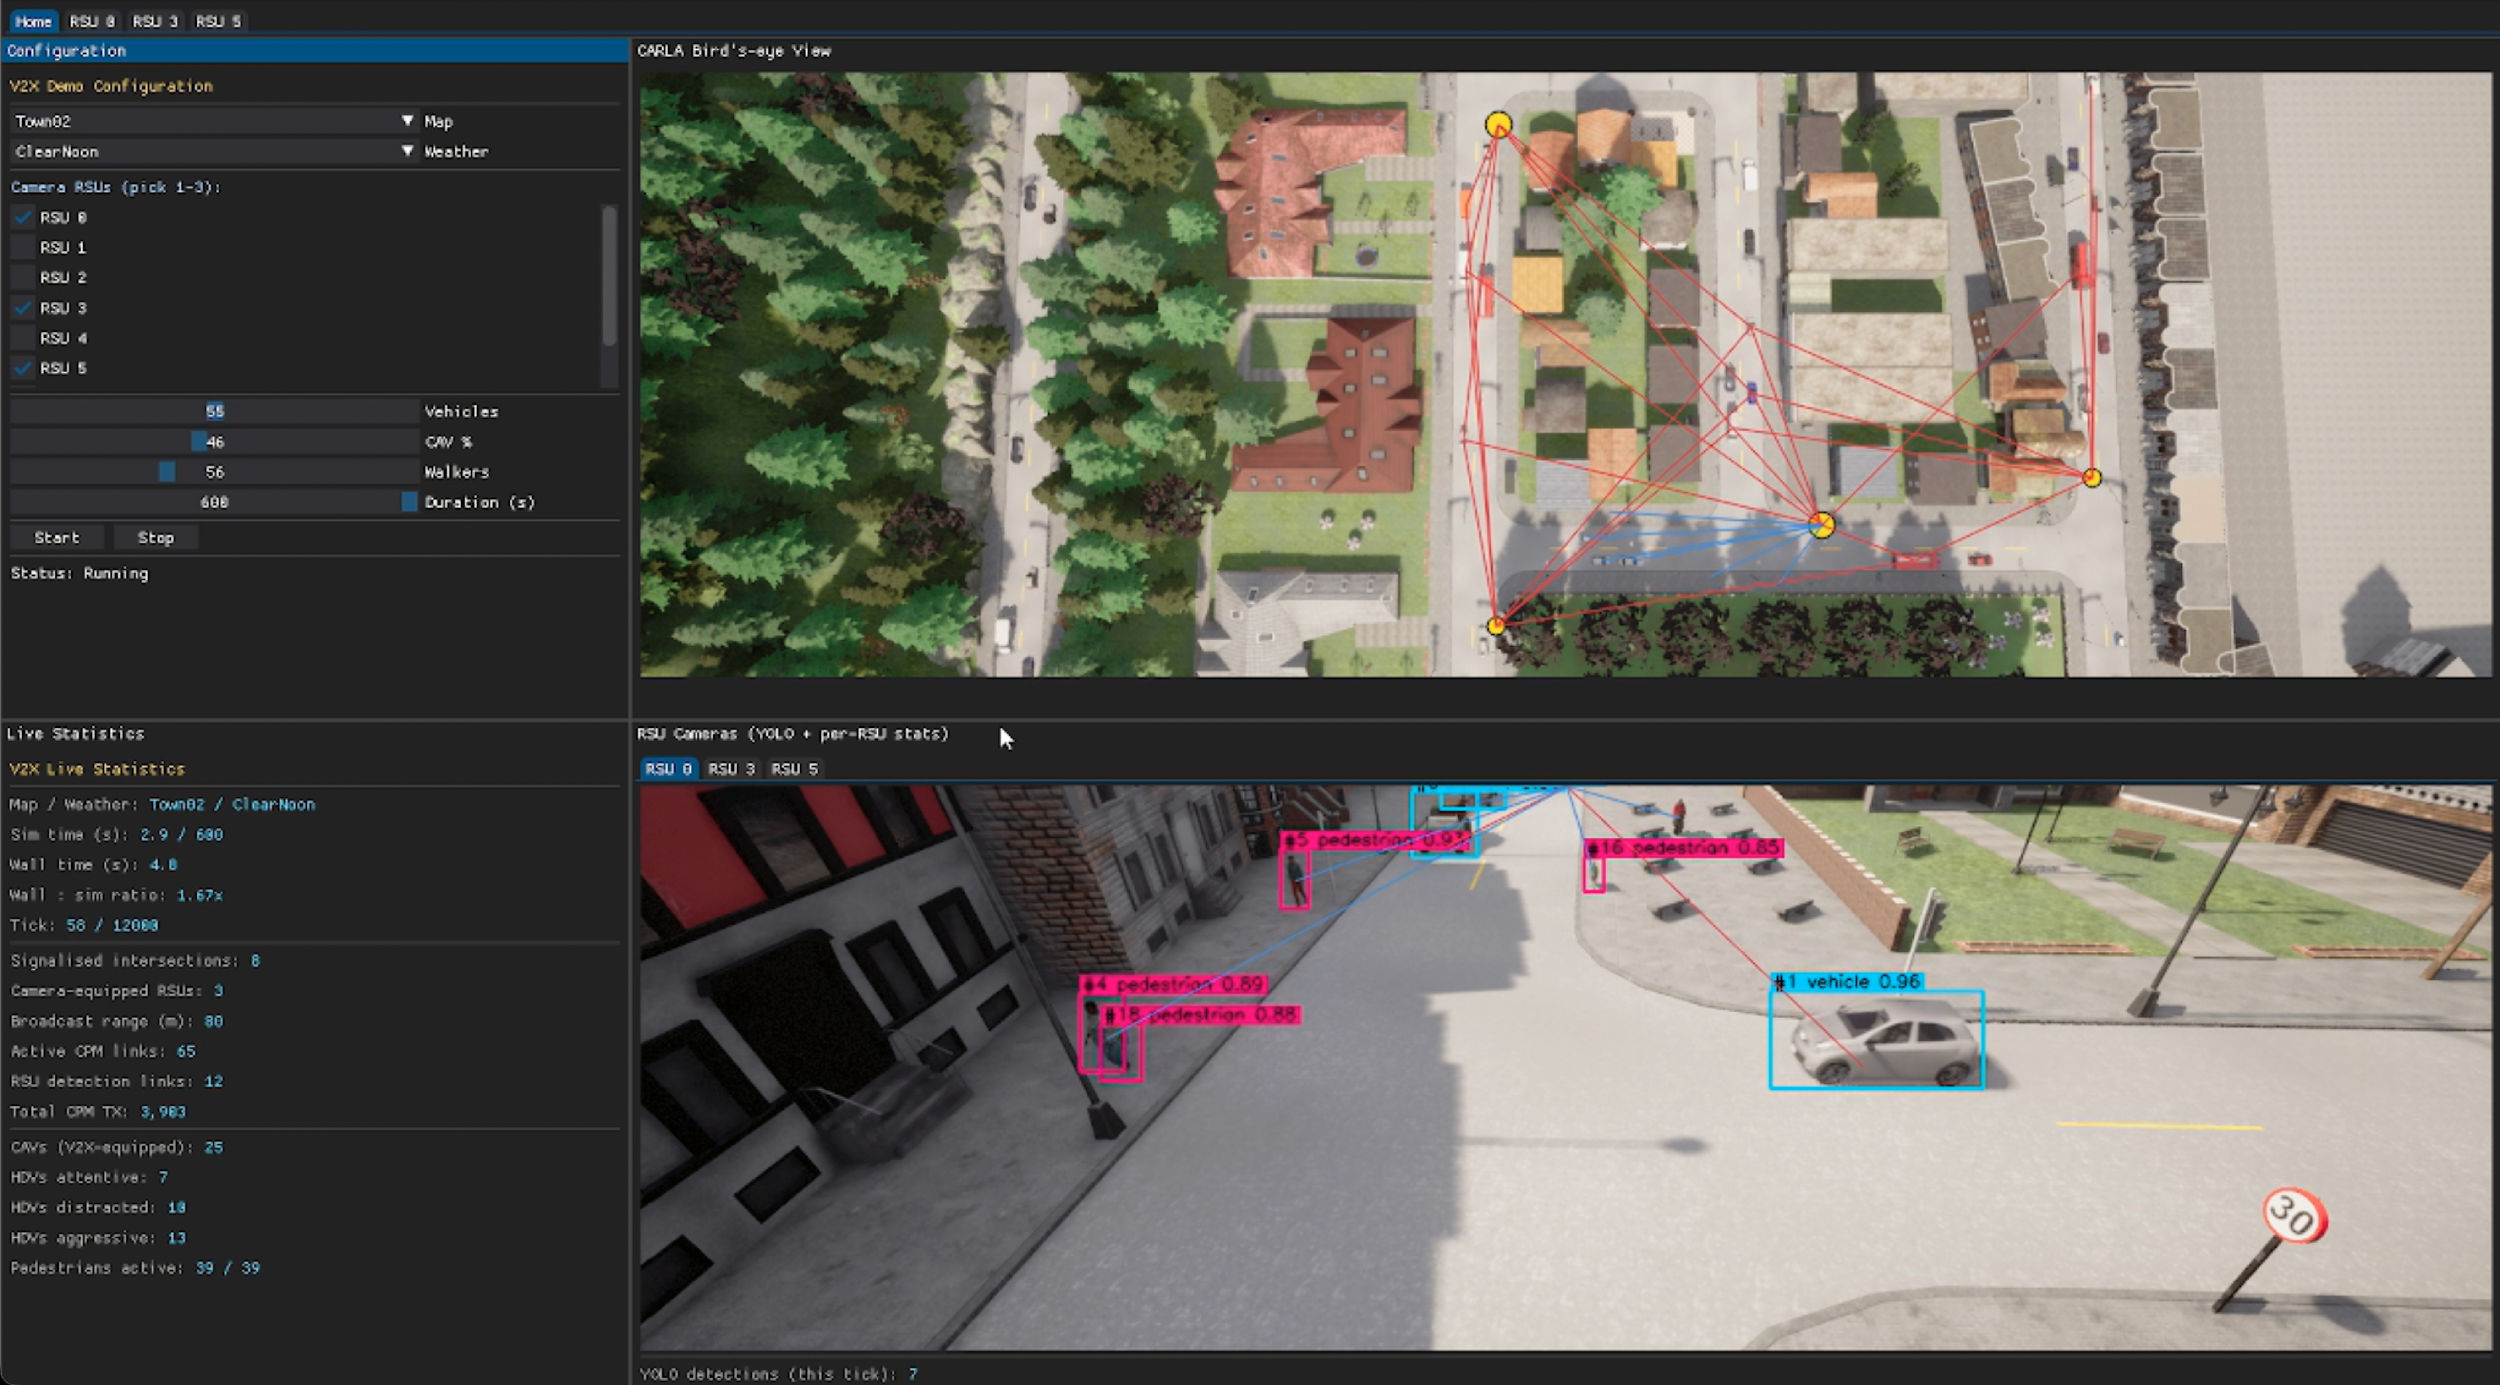
\includegraphics[width=\textwidth]{figA1-demo-ui-run1.png}
  \caption{Demonstration application, Run~1 (clear weather): configuration and live
  statistics panels (left), the bird's-eye view with RSU coverage rays (top-right),
  and an RSU camera with YOLO detections (bottom-right).}
  \label{fig:ui1}
\end{figure}

\begin{figure}[t]
  \centering
  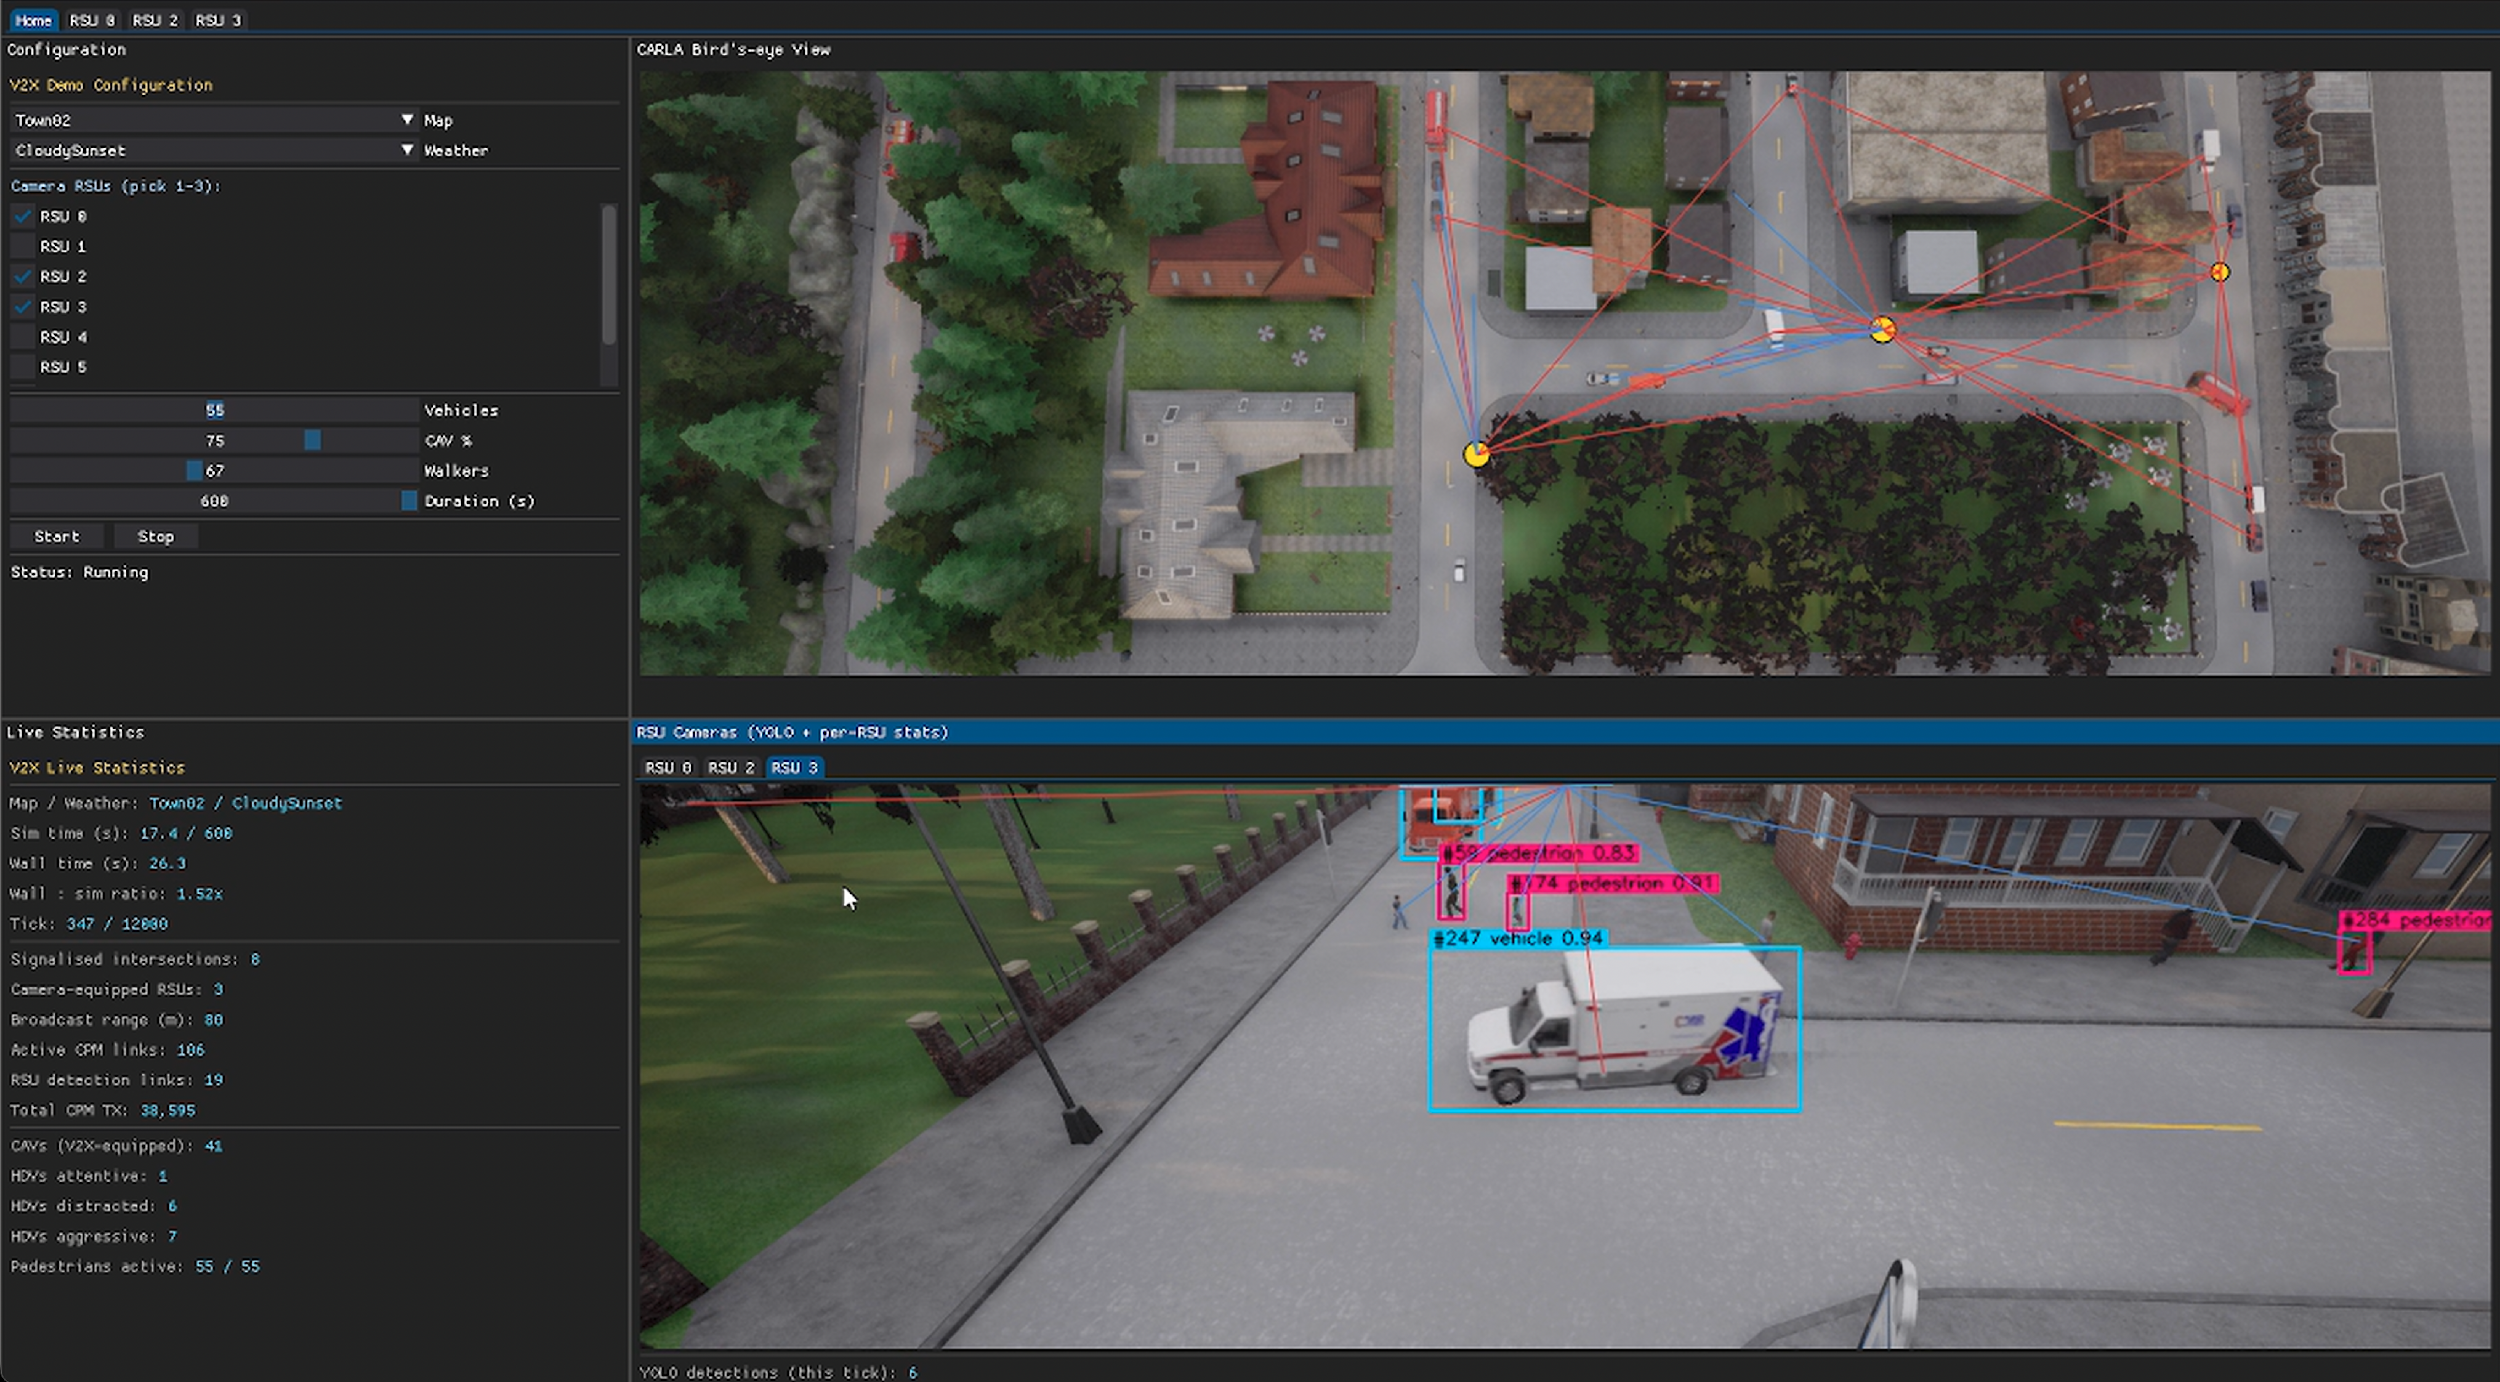
\includegraphics[width=\textwidth]{figA2-demo-ui-run2.png}
  \caption{Demonstration application, Run~2 (cloudy/sunset): three RSUs stream CPMs
  while YOLO detects a commercial vehicle at the junction.}
  \label{fig:ui2}
\end{figure}

\begin{figure}[t]
  \centering
  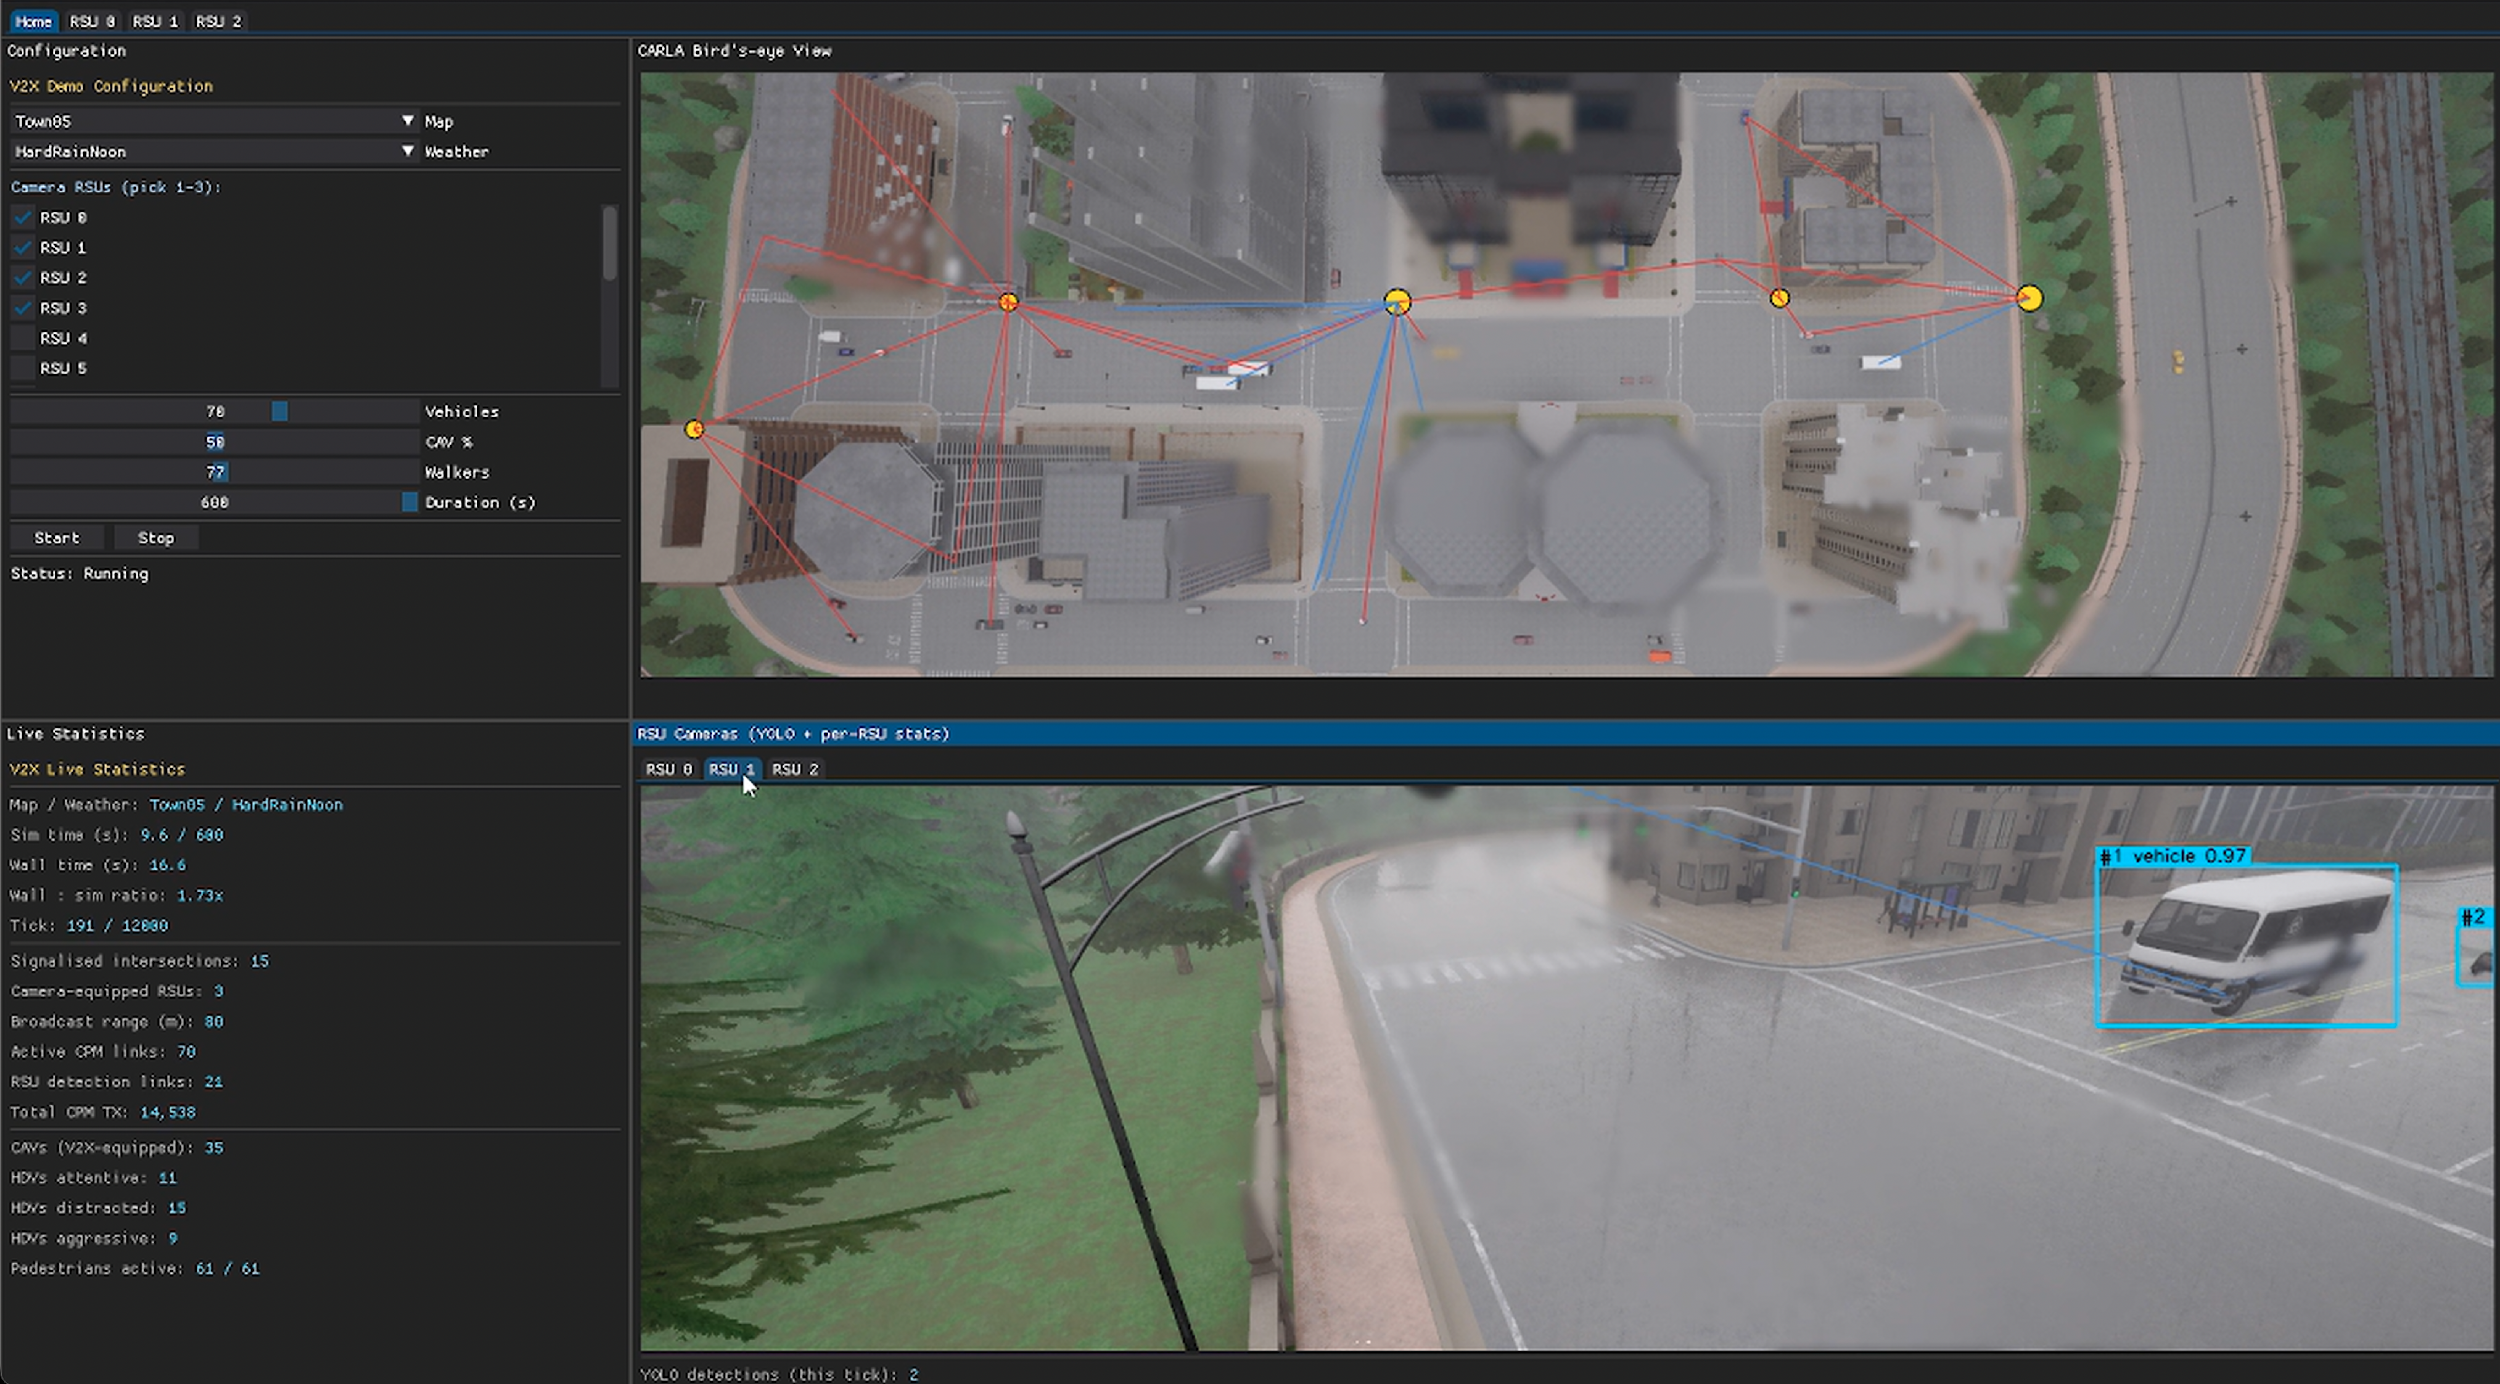
\includegraphics[width=\textwidth]{figA3-demo-ui-run3.png}
  \caption{Demonstration application, Run~3 (hard rain, downtown): detection and
  cooperative messaging continue on a wet road surface, with a bus detected in the
  RSU camera.}
  \label{fig:ui3}
\end{figure}

\end{document}
